\documentclass[a4paper]{article}

%% Language and font encodings
\usepackage[english]{babel}
\usepackage[utf8x]{inputenc}
\usepackage[T1]{fontenc}

%% Sets page size and margins
\usepackage[a4paper,top=3cm,bottom=2cm,left=2cm,right=2cm,marginparwidth=2cm]{geometry}

%% Useful packages
\usepackage{amsmath}
\usepackage{amsfonts}
\usepackage{bbm}
\usepackage{graphicx}
\usepackage[colorinlistoftodos]{todonotes}
\usepackage[colorlinks=true, allcolors=blue]{hyperref}
\usepackage{float}
\usepackage{enumerate}
\usepackage[export]{adjustbox}
\usepackage{mathrsfs}
\usepackage{subcaption}

\usepackage{tikz}
\usetikzlibrary{arrows}
\tikzset{
    vertex/.style={circle,draw,minimum size=1.5em},
    edge/.style={->,> = latex'}
}

\title{Stochastic Processes}
\author{Kevin Chang}

\graphicspath{ {./images/} }

\begin{document}
\maketitle

\section{Laplace Transform}
\begin{itemize}
    \item $\mathcal{L}\{f\}(s) = \int_0^\infty f(t) e^{-st} dt$
    \item Property
        \begin{itemize}
            \item $tf(t) \leftrightarrow -F'(s)$
            \item $\frac{f(t)}{t} \leftrightarrow \int_s^\infty F(\sigma) d \sigma$
            \item $f'(t) \leftrightarrow sF(s) - f(0^-)$
            \item $\int_0^t f(\tau) d\tau \leftrightarrow \frac{F(s)}{s}$
            \item $e^{at}f(t) \leftrightarrow F(s-a)$
            \item $f(t-a)u(t-a) \leftrightarrow e^{-at}F(s)$
        \end{itemize}
\end{itemize}

\section{Moment Generating Function}
\begin{itemize}
    \item Moment Generating Function: $\mathbb{E}[e^{tX}]$
        \begin{itemize}
            \item Property:
                \begin{itemize}
                    \item $\mathbb{E}[e^{tX}] = \int_{-\infty}^\infty e^{tx} f_X(x) dx$
                    \item $\mathbb{E}[e^{tX}] = \sum_{k=0}^\infty \mathit{E}[X^k] \frac{t^k}{k!}$
                        \begin{itemize}
                            \item $e^{tx} = \sum_{k=0}^\infty \frac{(tx)^k}{k!}$
                            \item $\mathit{E}[e^{tX}] = \mathit{E}[\sum_{k=0}^\infty \frac{(tX)^k}{k!}] = \sum_{k=0}^\infty \mathit{E}[X^k] \frac{t^k}{k!}$
                        \end{itemize}
                    \item $\frac{d\mathbb{E}[e^{tX}]}{dt} = \mathbb{E}[X]$
                    \item $\mathbb{E}[e^{t(aX+b)}] = e^tb\mathbb{E}[e^{taX}]$
                    \item Not all random variables have Moment generating function
                \end{itemize}
        \end{itemize}
    \item Characteristic Function: $\mathbb{E}[e^{itX}]$
        \begin{itemize}
            \item Property:
                \begin{itemize}
                    \item All random variables have Moment generating function
                \end{itemize}
        \end{itemize}
    \item Joint Moment Generating Function: $G(x, y) = \mathbb{E}[e^{xX}e^{yY}]$
    \item Property:
        \begin{itemize}
            \item (Joint) moment generating funciton uniquely determines the (joint) CDF
        \end{itemize}
    \item Example
        \begin{itemize}
            \item Trapped miner's random walk
                \begin{itemize}
                    \item Miner has probability of $\frac{1}{3}$ to waste 3 hours in vain, $\frac{1}{3}$ to waste 5 hours in vain, and $\frac{1}{3}$ to spend 2 hours to go out of the mine.
                    \item $X$ is the random variables of the hours to go out of the mine
                    \item $Y_i$ is the random variables of the hours for the $i$-th action.
                    \item $\mathbb{E}[e^{tX}] = \mathbb{E}[e^{tX}|Y_1 = 2] + \mathbb{E}[e^{tX}|Y_1 = 3] + \mathbb{E}[e^{tX}|Y_1 = 5]$

                        $= \mathbb{E}[e^{2t}] + \mathbb{E}[e^{t(X+3)}] + \mathbb{E}[e^{t(X+5)}]$
                    \item Find expectation and variance by joint moment generating function
                \end{itemize}
        \end{itemize}
\end{itemize}

\section{Expectation}
\begin{itemize}
    \item $N$ i.i.d. events, when $N$ is a random variable
        \begin{itemize}
            \item Suppose $N$ is a integer random variable
            \item Suppose $X_1, \dots, X_i, \dots, X_N$ are i.i.d random variables with mean $\mu$ and variance $\sigma^2$
            \item $Y = \sum_{i = 1}^N X_i$
            \item $\mathbb{E}[Y] = \mathbb{E}[N] \mu$
                \begin{itemize}
                    \item $\mathbb{E}[Y] = \sum_{n = 1}^\infty \mathbb{E}[\sum_{i = 1}^N X_i|N=n] P[N=n]$

                        $= \mu \times \sum_{n=1}^\infty n P[N=n] = \mathbb{E}[N] \mu$
                \end{itemize}
            \item $\mathbb{E}[Y^2] = \mathbb{E}[N] \mathbb{E}[X^2] + \mathbb{E}[N^2] \mu^2 - \mathbb{E}[N] \mu^2$
                \begin{itemize}
                    \item $\mathbb{E}[Y^2] = \sum_{n = 1}^\infty \mathbb{E}[(\sum_{i = 1}^N X_i)^2|N=n] P[N=n]$
                        $= \sum_{n = 1}^\infty (n \mathbb{E}[X_i^2] + n(n-1)\mu^2) P[N=n]$

                        $= \mathbb{E}[N] \mathbb{E}[X^2] + \mathbb{E}[N^2] \mu^2 - \mathbb{E}[N] \mu^2$
                \end{itemize}
            \item $\mathit{Var}(Y) = \mathbb{E}[N]\sigma^2 + \mathit{Var}(N)\mu^2$
        \end{itemize}
    \item Expectation by $P[X>x]$
        \begin{itemize}
            \item $\mathbb{E}[X] = \sum_x P[X > x]$, when $X$ is a non-negative discrete random variable
                \begin{itemize}
                    \item $\mathbb{E}[X] = \sum_{x=0}^\infty x P[X = x] = \sum_{x=0}^\infty \sum_{y=0}^{x-1} P[X = x] = \sum_{y=0}^\infty \sum_{x=y + 1}^\infty P[X = x] = \sum_{y = 0}^\infty P[X > y]$
                \end{itemize}
            \item $\mathbb{E}[X] = \int_0^\infty P[X > x] dx$, when $X$ is a non-negative continuous random variable
                \begin{itemize}
                    \item $\mathbb{E}[X] = \int_0^\infty x f_X(x) dx = \int_0^\infty \int_0^x f_X(x) dy dx = \int_0^\infty \int_y^\infty f_X(x) dx dy = \int_0^\infty P[X > y] dy$
                \end{itemize}
        \end{itemize}
\end{itemize}

\section{Inequality}
\begin{itemize}
    \item Markov Inequality

        Definition:
        \begin{itemize}
            \item Suppose $X \geq 0$, then $P[X \geq \epsilon] \leq \frac{\mathbb{E}[X]}{\epsilon}$
        \end{itemize}

        Proof:
        \begin{enumerate}
            \item $\mathbb{E}[X] = \int_0^\infty x f_X(x) \geq \int_\epsilon^\infty x f_X(x) \geq \epsilon \int_\epsilon^\infty f_X(x) = \epsilon P[X \geq \epsilon]$
            \item $X(\omega) \geq \epsilon \mathbbm{1}_{X(\omega) \geq \epsilon}, \forall \omega \in S$
                \begin{itemize}
                    \item Calculate expectation on both side.
                    \item $\mathbb{E}[X] \geq \epsilon P[X \geq \epsilon]$
                \end{itemize}
        \end{enumerate}
        Property:
        \begin{itemize}
            \item The equality happens when $P[X=k] = 0, \forall k \not \in \{0, \epsilon\}$.
        \end{itemize}
    \item Chebyshev Inequality

        Definition:
        \begin{itemize}
            \item Suppose $m = \mathbb{E}[X], \sigma^2 = \mathit{Var}(X)$, then $P[|X - m| \geq \epsilon] \leq \frac{\sigma^2}{\epsilon^2}$
        \end{itemize}
        Proof:
        \begin{itemize}
            \item $P[|X - m| \geq \epsilon] = P[(X - m)^2 \geq \epsilon^2]$
            \item $P[(X - m)^2 \geq \epsilon^2] \leq \frac{\mathbb{E}[(X-m)^2]}{\epsilon^2}$ (by Markov Inequality)
        \end{itemize}
        Property:
        \begin{itemize}
            \item The equality happens when $P[X = k] = 0, \forall k \not \in \{m - \epsilon , m , m + \epsilon\}$.
            \item Might be tighter than Markov Inequality since it requires $m, \sigma$
        \end{itemize}
    \item Chernoff Inequality

        Definition:
        \begin{itemize}
            \item Suppose $X_1, \dots, X_n$ are independent identically distributed Bernoulli random variable with probability $p$ and $X = \sum_{i=1}^n X_i$
            \item $P[X \geq \epsilon] \leq \frac{(pe^{t} + 1 - p)^n}{e^{t\epsilon}} \leq \frac{e^{np(e^{t} - 1)}}{e^{t\epsilon}}$
                \begin{itemize}
                    \item $P[X \geq \epsilon] = P[e^{tX} \geq e^{t\epsilon}] \leq \frac{E[e^{tX}]}{e^{t\epsilon}} = \frac{(E[e^{tX_i}])^n}{e^{t\epsilon}} = \frac{(pe^{t} + 1 - p)^n}{e^{t\epsilon}} \leq \frac{e^{np(e^{t} - 1)}}{e^{t\epsilon}}$
                \end{itemize}
            \item $P[X \geq np(1 + \epsilon)] \leq (\frac{e^{\epsilon}}{(1+\epsilon)^{1 + \epsilon}})^{np} \leq \left\{ \begin{array}{ll} e^{\frac{-\epsilon^2 np}{3}} & \text{ if } 0 \leq \epsilon \leq 1 \\ e^{\frac{-\epsilon^2 np}{(2 + \epsilon)}} & \text{ if } \epsilon \geq 1 \end{array} \right.$
                \begin{itemize}
                    \item Substitude $\epsilon$ with $np(1+\epsilon)$
                    \item Substitude $t$ with $\log(1+\epsilon)$
                    \item the last inequality is without proof
                \end{itemize}
            \item $P[X \leq \epsilon] \leq \frac{(pe^{t} + 1 - p)^n}{e^{t\epsilon}} \leq \frac{e^{np(e^{t} - 1)}}{e^{t\epsilon}}$
                \begin{itemize}
                    \item $P[X \leq \epsilon] = P[e^{-tX} \geq e^{-t\epsilon}] \leq \frac{E[e^{-tX}]}{e^{-t\epsilon}} = \frac{(E[e^{-tX_i}])^n}{e^{-t\epsilon}} = \frac{(pe^{-t} + 1 - p)^n}{e^{-t\epsilon}} \leq \frac{e^{np(e^{-t} - 1)}}{e^{-t\epsilon}}$
                \end{itemize}
            \item $P[X \leq np(1 - \epsilon)] \leq (\frac{e^{-\epsilon}}{(1-\epsilon)^{1 - \epsilon}})^{np} \leq e^{\frac{-\epsilon^2 np}{2}}$
                \begin{itemize}
                    \item Substitude $\epsilon$ with $np(1-\epsilon)$
                    \item Substitude $t$ with $- \log(1-\epsilon)$
                    \item the last inequality is without proof
                \end{itemize}
        \end{itemize}
    \item Chernoff/ Hoeffding Lemma

        Definition:
        \begin{itemize}
            \item Suppose $X_1, \dots, X_n$ are independent distributed random variable and $a_i \leq X_i \leq b_i$
            \item Suppose $X = \sum_{i=1}^n X_i$ and $\mu = \mathbb{E}[X]$
            \item $P[|X-\mu| \geq \epsilon] \leq 2 e^{\frac{-2\epsilon^2}{\sum_{i=1}^n(b_i - a_i)^2}}$ without proof
        \end{itemize}
    \item Application:
        \begin{itemize}
            \item Balls in Bins

                Definition: Throw $n$ balls into $n$ bins, find bounds for the maximum number of balls in all bins
                \begin{itemize}
                    \item $P[\text{ maximum number of balls in all bins } \geq \epsilon]$

                        $= P[\cup_{i=1}^n \text{ number of balls in $i$-th bin } \geq \epsilon]$

                        $\leq n \times P[\text{ number of balls in one bin } \geq \epsilon]$
                    \item By Markov inequality:
                        \begin{itemize}
                            \item $P[\text{ number of balls in one bin } \geq \epsilon] \leq \frac{1}{\epsilon} \rightarrow$ useless
                        \end{itemize}
                    \item By Chebyshev inequality:
                        \begin{itemize}
                            \item $P[\text{ number of balls in one bin } \geq \epsilon] \leq \frac{(1-\frac{1}{n})}{\epsilon^2}$
                            \item $P[\text{ maximum number of balls in all bins } \geq n^{\frac{1}{2} + \epsilon}] \leq \frac{(1-\frac{1}{n})}{n^{2\epsilon}}$
                            \item when $n \rightarrow \infty$, the maximum number of balls should less than $n^{\frac{1}{2} + \epsilon}$
                        \end{itemize}
                    \item By Chernoff inequality:
                        \begin{itemize}
                            \item $P[\text{ number of balls in one bin } \geq 2 \log n] \leq \frac{e^{np(e^{t} - 1)}}{n^{2t}}$
                            \item $P[\text{ maximum number of balls in all bins } \geq 2 \log n] \leq \frac{e^{np(e^{t} - 1)}}{n^{2t - 1}}$
                            \item when $t$ is a constant $\geq 0.5$ and $n \rightarrow \infty$, the maximum number of balls should less than $2 \log n$
                        \end{itemize}
                \end{itemize}
        \end{itemize}
\end{itemize}

\section{Law of Large Numbers}
\begin{itemize}
    \item $\{X_i\}_{i = 1}^\infty$ is a sequence of pairwise uncorrelated random variable with

        $\mathbb{E}[X_i] = m, \mathit{Var}(X_i) = \sigma_i^2$.
    \item $M_n = \frac{1}{n}\sum_{i = 1}^n X_i$
    \item $M_n \rightarrow m$ almost surely, in mean square and in probability.
\end{itemize}

\section{Memoryless}
\begin{itemize}
    \item Definition: $P[X > x_1 + x_2 | X > x_1] = P[X > x_2]$
    \item Property:
        \begin{itemize}
            \item Exponential random variable is the only continuous memoryless random variable
            \item Bernoulli random variable is the only discrete memoryless random variable
        \end{itemize}
\end{itemize}

\section{Famous Random Variable}
\begin{itemize}
    \item Poisson:

        $P[X=k] = \frac{\lambda^k}{k!}\exp(-\lambda)$

        $\mathbb{E}[X] = \sum_{k=0}^\infty k\frac{\lambda^k}{k!}\exp(-\lambda)$
        $= \sum_{k=0}^\infty \lambda \frac{\lambda^{k-1}}{(k-1)!}\exp(-\lambda) = \lambda$

        Interpretation:
        \begin{itemize}
            \item Cut total time into infinite period in Binomial random variable, $n \rightarrow \infty, p \rightarrow \frac{\lambda}{n}$

            \item $\rightarrow P[X=k] = \lim_{n\rightarrow \infty} \binom{n}{k}(\frac{\lambda}{n})^k(\frac{n-\lambda}{n})^{n-k} = \frac{\lambda^k}{k!}(1-\frac{\lambda}{n})^{n} = \frac{\lambda^k}{k!}\exp(-\lambda)$
        \end{itemize}
    \item Gaussian: $N(m, \sigma^2)$
        \begin{itemize}
            \item $f_X[x] = \frac{1}{\sqrt{2\pi\sigma^2}}e^{\frac{-(x-m)^2}{2\sigma^2}}, \forall x \in \mathbb{R}$
            \item $\mathbb{E}[e^{cX}] = e^{cm + \frac{c^2\sigma^2}{2}}$
        \end{itemize}
    \item Erlang:

        $f_X(x) = \frac{\lambda^n x^{n-1} e^{-\lambda x}}{(n-1)!}, \forall x \in \mathbb{R}$

        $\mathbb{E}[X] = \frac{n}{\lambda}$

        Interpretation:
        \begin{itemize}
            \item Suppose $X_1, X_2, ..., X_n$ are i.i.d exponential random variable with $\lambda$.
            \item $X = \sum_{i = 1}^n X_i$
            \item Proof by induction:

                Suppose $n = 2$, 
                $f_X(x) = \int_0^x \lambda e^{-\lambda t} \lambda e^{-\lambda(x - t)} dt$
                $= \lambda^2 x e^{-\lambda x}$
        \end{itemize}
\end{itemize}

\section{Stochastic Processes}
\begin{itemize}
    \item Stochastic Process: a collection of random variable $X(t)$

        General Stochastic Process
        \begin{itemize}
            \item Central Limit Theorem
                \begin{itemize}
                    \item Sum of i.i.d. stochastic process converge to Gaussian Process
                \end{itemize}
        \end{itemize}
        Arrival Process: a sequence of arriving event in continuous time
\begin{figure} [H]
    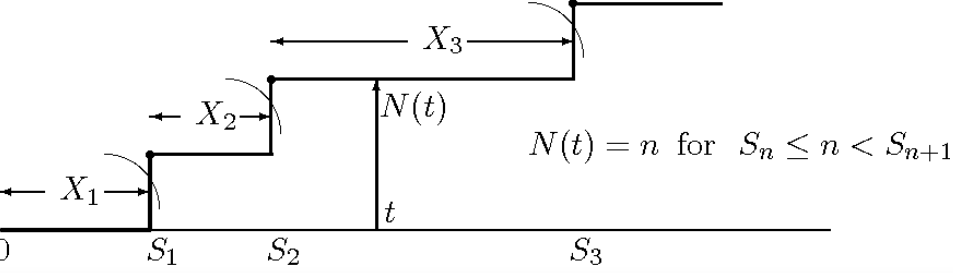
\includegraphics[width=0.5\linewidth, center]{image/arrival_process.png}
\end{figure}
        \begin{itemize}
            \item $X_i$: the time between the $i$-th event and the $i-1$-th event
            \item $S_i$: the time from start to $i$-th event
            \item $N(t)$: the number of the arrived event at time $t$
            \item $X$ and $S$ Relation:
                \begin{itemize}
                    \item $X_1 = S_1, X_i = S_i - S_{i-1}$
                \end{itemize}
            \item $N$ and $S$ Relation:
                \begin{itemize}
                    \item $N(t) < n \leftrightarrow S_{n+1} > t$
                    \item $N(t) \geq n \leftrightarrow S_n \leq t$
                    \item $N(t) = n \leftrightarrow S_n \leq t < S_{n+1}$
                    \item $N(t) = \max \{n: S_n \leq t\}$
                \end{itemize}
            \item Renewal Process: an arrival process with i.i.d $X_i$

                Delayed Renewal Process: the process becomes a renewal process after several arrivals

                $X_i$ Property
                \begin{itemize}
                    \item if $X_i$ is dependent on the interval states, then $X_i$ might be dependent on $X_{i-1} \rightarrow$ not renewal process
                \end{itemize}
                $S_i$ Property
                \begin{itemize}
                    \item $P[\lim_{n \rightarrow \infty} S_n = \infty] = 1$

                        Proof: $\lim_{n \rightarrow \infty} P[S_n = \infty] = \lim_{n \rightarrow \infty} P[\sum_{i = 1}^n X_n = n \times \mathbb{E}[X_i]] = 1$

                        Interpretation: infinite events do not take finite time
                \end{itemize}
                $N(t)$ Property
                \begin{itemize}
                    \item for any $t, P[N(t) < \infty] = 1$

                        Proof: $P[\lim_{n \rightarrow \infty} S_n = \infty] = 1 \rightarrow$ for any $t, P[\lim_{n \rightarrow \infty} S_{n+1} > t] = 1$

                        Interpretation: infinite events do not take finite time
                    \item $P[\lim_{t \rightarrow \infty} N(t) \rightarrow \infty] = 1$

                        Proof: if $P[\lim_{t \rightarrow \infty} N(t) = k] > 0 \rightarrow P[X_{k+1} = \infty] > 0$

                        Interpretation: finite events do not take infinite time
                    \item $P[\lim_{t \rightarrow \infty} \frac{N(t)}{t} = \frac{1}{\mathbb{E}[X_i]}] = 1$

                        Proof: $P[\lim_{t \rightarrow \infty} \frac{N(t)}{S_{N(t) + 1}} \leq \lim_{t \rightarrow \infty} \frac{N(t)}{t}] = 1$ and $P[\lim_{t \rightarrow \infty} \frac{N(t)}{S_{N(t) + 1}} = \frac{1}{\mathbb{E}[X_i]}] = 1$

                        $P[\lim_{t \rightarrow \infty} \frac{N(t)}{t} \leq \lim_{t \rightarrow \infty} \frac{N(t)}{S_{N(t)}}] = 1$ and $P[\lim_{t \rightarrow \infty} \frac{N(t)}{S_{N(t)}} = \frac{1}{\mathbb{E}[X_i]}] = 1$
                \end{itemize}
                Inspection Paradox
                \begin{itemize}
                    \item $\mathbb{E}[X_{N(t) + 1}] \geq \mathbb{E}[X_i]$: inspection paradox

                        Interpretation:
                        \begin{itemize}
                            \item $f_{X_{N(t)+1}}(x) = \lambda x f_{X_i}(x)$
                            \item when selecting $t$ with equal probability, we tend to choose $X_i$ with longer period
                        \end{itemize}
                    \item $P[\lim_{t \rightarrow \infty} \frac{1}{t} \int_0^t (S_{N(t) + 1} - s) ds = \frac{\mathbb{E}[X_i^2]}{2\mathbb{E}[X_i]}] = 1$

                        Proof:

                        $P[\lim_{t \rightarrow \infty} \frac{1}{t} \sum_{i = i}^{N(t)} \frac{\mathbb{E}[X_i^2]}{2} \leq \lim_{t \rightarrow \infty} \frac{1}{t} \int_0^t (S_{N(t) + 1} - s) ds] = 1$ and $P[\lim_{t \rightarrow \infty} \frac{1}{t} \sum_{i = i}^{N(t)} \frac{\mathbb{E}[X_i^2]}{2} = \frac{\mathbb{E}[X_i^2]}{2\mathbb{E}[X_i]}] = 1$

                        $P[\lim_{t \rightarrow \infty} \frac{1}{t} \int_0^t (S_{N(t) + 1} - s) ds \leq \lim_{t \rightarrow \infty} \frac{1}{t} \sum_{i = i}^{N(t) + 1} \frac{\mathbb{E}[X_i^2]}{2}] = 1$ and $P[\lim_{t \rightarrow \infty} \frac{1}{t} \sum_{i = i}^{N(t) + 1} \frac{\mathbb{E}[X_i^2]}{2} = \frac{\mathbb{E}[X_i^2]}{2\mathbb{E}[X_i]}] = 1$
                    \item $P[\lim_{t \rightarrow \infty} \frac{1}{t} \int_0^t (s - S_{N(t)}) ds = \frac{\mathbb{E}[X_i^2]}{2\mathbb{E}[X_i]}] = 1$

                        Proof: similar to above
                    \item $P[\lim_{t \rightarrow \infty} \frac{1}{t} \int_0^t X_{N(t)} ds = \frac{\mathbb{E}[X_i^2]}{\mathbb{E}[X_i]}] = 1$

                        Proof: $P[\lim_{t \rightarrow \infty} \frac{1}{t} \int_0^t X_{N(t)} ds = \lim_{t \rightarrow \infty} \frac{1}{t} \int_0^t (S_{N(t) + 1} - S_{N(t)}) ds] = 1$
                    \item $\mathbb{E}[X_{N(t) + 1}] = \frac{\mathbb{E}[X_i^2]}{\mathbb{E}[X_i]}$

                        Proof: $P[\lim_{t \rightarrow \infty} \frac{1}{t} \int_0^t X_{N(t)} ds = \frac{\mathbb{E}[X_i^2]}{\mathbb{E}[X_i]}] = P[\mathbb{E}[X_{N(t) + 1}] = \frac{\mathbb{E}[X_i^2]}{\mathbb{E}[X_i]}] = 1$
                \end{itemize}
                Central Limit Theorem
                \begin{itemize}
                    \item $\mu = \mathbb{E}[X_i]$
                    \item $\sigma = \sqrt{\mathit{Var}(X_i)}$
                    \item $Z \sim$ Normal(0,1)
                    \item $\lim_{t \rightarrow \infty} P[N(t) \leq \frac{t}{\mu} + k \frac{\sigma \sqrt{t}}{\sqrt{\mu}^3}] = P[Z \leq k]$

                        Proof:
                        \begin{enumerate}
                            \item Suppose $n(t) = \frac{t}{\mu} + k \frac{\sigma \sqrt{t}}{\sqrt{\mu}^3}$
                            \item $P[N(t) \geq n(t)] = P[S_{n(t)} \leq t] = P[\frac{S_{n(t)} - n\mu}{\sigma \sqrt{n}} \leq \frac{t - n\mu}{\sigma \sqrt{n}}]$.
                            \item When $t \rightarrow \infty$, $\frac{t - n\mu}{\sigma \sqrt{n}} \rightarrow k$
                            \item By law of large number, $\lim_{t \rightarrow \infty} P[\frac{S_{n(t)} - n\mu}{\sigma \sqrt{n}} \leq k] = P[Z \leq k]$
                        \end{enumerate}
                        Interpretation:
                        \begin{itemize}
                            \item $\frac{t}{\mu}$ is approximately the mean of $N(t)$
                            \item $k \frac{\sigma \sqrt{t}}{\sqrt{\mu}^3}$ is $k\sigma \sqrt{n}$ after dividing by $\mu$, the ratio between $t$ and $N(t)$ and changing $n$ with $\frac{t}{\mu}$
                        \end{itemize}
                \end{itemize}
                Wald's Identity
                \begin{itemize}
                    \item Stopping Times: a random variable $\tau$ s.t. $\{\tau = n\}$ is independent of $\{X_i\}_{i=n+1}^\infty$
                    \item Stopping Condition: a condition to stop if we can consider $\tau = \min\{n: \text{ condition}(n) = \top \}$
                    \item Example: $N(t) + 1$ is a stopping times and can be consider $N(t) + 1 = \min\{n: S_n > t\}$
                    \item $\mathbb{E}[\sum_{i=1}^\tau X_i] = \mathbb{E}[\tau] \mathbb{E}[X_i]$ if $\mathbb{E}[X_i] < \infty$ and $\mathbb{E}[N] < \infty$

                        Proof:
                        \begin{enumerate}
                            \item $\mathbb{E}[\sum_{i=1}^\tau X_i] = \sum_{i=1}^\infty \mathbb{E}[X_i \times \mathbbm{1}_{i\leq \tau}]$ (by Fubin's Theorem without proof)

                               (if $\mathbb{E}[X_i] < \infty$ and $\mathbb{E}[N] < \infty$)
                            \item $\sum_{i=1}^\infty \mathbb{E}[X_i \times \mathbbm{1}_{i\leq \tau}] = \mathbb{E}[X_i] \sum_{i=1}^\infty \mathbb{E}[\mathbbm{1}_{i\leq \tau}]$ (by $P[\tau \geq i] = 1 - P[\tau < i]$ is independent of $X_i$)
                            \item $\mathbb{E}[X_i] \sum_{i=1}^\infty \mathbb{E}[\mathbbm{1}_{i\leq \tau}] = \mathbb{E}[\tau] \mathbb{E}[X_i]$
                        \end{enumerate}
                    \item $\lim_{t \rightarrow \infty} \frac{\mathbb{E}[N(t)]}{t} = \frac{1}{\mathbb{E}[X_i]}$

                        Proof:
                        \begin{itemize}
                            \item Suppose $\mu = \mathbb{E}[X_i]$
                            \item $\frac{\mathbb{E}[N(t)]}{t} = \frac{\mathbb{E}[S_{N(t) + 1}]}{t \times \mu} - \frac{1}{t}$ (by considering $N(t) + 1$ as the stopping time)
                            \item $\lim_{t \rightarrow \infty} \frac{\mathbb{E}[N(t)]}{t} \geq \frac{1}{\mu}$ (by $\mathbb{E}[S_{N(t) + 1}] > t$)
                            \item Suppose $\hat{X}_n = \min\{X_n, T\}$, where $T$ is a constant
                            \item $\frac{\mathbb{E}[N(t)]}{t} \leq \frac{\mathbb{E}[\hat{N}(t)]}{t} = \frac{\mathbb{E}[S_{\hat{N}(t) + 1}]}{t \times \hat{\mu}} - \frac{1}{t} \leq \frac{t+T}{t \times \hat{\mu}} - \frac{1}{t}$
                            \item $\lim_{n = \sqrt{t}, t \rightarrow \infty} \frac{\mathbb{E}[N(t)]}{t} \leq \frac{1}{\mu}$
                        \end{itemize}
                \end{itemize}
                Blackwell's Theorem
                \begin{itemize}
                    \item $\mathbb{E}[N(t)] = F_{X_i}(t) + \int_0^t \mathbb{E}[N(t-x)] f_{X_i}(t) dt$

                        Proof:
                        $\mathbb{E}[N(t)] = \int_0^t \mathbb{E}[N(t)|X_1 = x] f_{X_1}(x) dx$

                        $= \int_0^t \mathbb{E}[N(t-x) + 1] f_{X_1}(x) dx$
                        $= F_{X_i}(t) + \int_0^t \mathbb{E}[N(t-x)] f_{X_i}(t) dt$
                    \item $\mathcal{L}\{\mathbb{E}[N(t)]\}(s) = \frac{\mathcal{L}\{f_{X_i}\}(s)}{s(1 - \mathcal{L}\{f_{X_i}\}(s))}$

                        Proof: Laplace transform both sides
                    \item Lattice/ Non-Lattice: $N(t)$ is lattice iff $X_i$ only takes on values that are $nd, n \in \mathbb{N}, d \in \mathbb{R}$
                    \item For a non-lattice process: $\lim_{t \rightarrow \infty} \mathbb{E}[N(t + \delta) - N(t)] = \frac{\delta}{\mathbb{E}[X_i]}$, for any $\delta$

                        Proof: Without Proof

                        Interpretation: $\mathbb{E}[N(t)]$ will converge to be linear
                    \item For a lattice process and period $d$: $\lim_{n \rightarrow \infty} \mathbb{E}[\text{\# events at $t = nd$}] = \frac{d}{\mathbb{E}[X_i]}$

                        Proof: Without Proof

                        Interpretation: $\mathbb{E}[N(t)]$ will converge to be stairs with width $d$ and height $\frac{d}{\mathbb{E}[X_i]}$
                \end{itemize}
            \item Renewal-Reward Process:

                Definition
                \begin{itemize}
                    \item A renewal process $N(t)$ and $\{R_i\}_{i = 1}^\infty$ such that $(X_i, R_i)$ are i.i.d.

                        ($X_i, R_j, i \not = j$ are independent, but $X_i, R_i$ might be dependent)
                \end{itemize}
                Property
                \begin{itemize}
                    \item $P[\lim_{t \rightarrow \infty} \frac{1}{t} \sum_{i=1}^{N(t)} R_i = \frac{\mathbb{E}[R_i]}{\mathbb{E}[X_i]}] = 1$

                        Proof: $P[\lim_{t \rightarrow \infty} \frac{1}{t} \sum_{i=1}^{N(t)} R_i = \lim_{t \rightarrow \infty} \sum_{i=1}^{N(t)} \frac{R_i}{N(t)} \times \lim_{t \rightarrow \infty} \frac{N(t)}{t}] = 1$
                \end{itemize}
            \item Poisson Process: a renewal process with $X_i \sim \text{Exponential}(\lambda)$

                $S_i$ Property
                \begin{itemize}
                    \item $S_i$ is an Erlang random variable

                        Erlang is the sum of the Exponential random variables
                    \item Joint Distribution $f_{S_1, \dots, S_n}(s_1, \dots, s_n) = \lambda^n e^{-\lambda s_n}$

                        Prove by induction.

                        Induce by $f_{S_1, \dots, S_n}(s_1, \dots, s_n) = f_{S_1, \dots, S_{n-1}}(s_1, \dots, s_{n-1}) \times f_{S_n | S_1, \dots, S_{n-1}}(s_n, s_1, \dots, s_{n-1})$
                \end{itemize}
                $N(t)$ Property
                \begin{itemize}
                    \item $N(t) \sim \text{Poisson}(\lambda t), P[N(t) = n] = \frac{(\lambda t)^n}{n!}e^{-\lambda t}$ 

                        Prove by $P[N(t) = n] = P[S_n \leq t \text{ and } S_{n+1} > t]$
                    \item Conditioned on $N(t) = n$, the set of arrival times $\{s_1, \dots, s_n\}$ have the same distribution with a set of $n$ sorted i.i.d. Uniform$(0, t)$ random variables

                        Prove by $f_{S_1, \dots, S_n | N(t)}(s_1, \dots, s_n, n) = \frac{f_{S_1, \dots, S_n}(s_1, \dots, s_n) P[X_{n+1} > t - s_n]}{P[N(t) = n]} = \frac{n!}{t^n}$
                \end{itemize}
                Property
                \begin{itemize}
                    \item $Z$ is the interval from $t$ to the first arrival $\rightarrow Z$ is exponential random variable with same $\lambda$ and independent of $N(t)$ and the arrival time before $t$

                        Proof:

                        $P[Z > z] = \sum_{n = 0}^\infty \int_0^\infty \dots \int_0^\infty P[Z>z|N(t) = n, S_1 = s_1, \dots, S_n = s_n] ds_1 \dots ds_n$

                        $= \sum_{n = 0}^\infty \int_0^\infty \dots \int_0^\infty P[X_{n+1}>z+t-s_n|N(t) = n, S_1 = s_1, \dots, S_n = s_n] ds_1 \dots ds_n$

                        $= \sum_{n = 0}^\infty \int_0^\infty \dots \int_0^\infty P[X_{n+1}>z+t-s_n|X_{n+1} > t-s_n] ds_1 \dots ds_n = e^{-\lambda z}$
                    \item Stationary Increments: $N(t_1 + t_2) - N(t_1)$ and $N(t_2)$ share the same distribution

                        Without Proof
                    \item Independent Increments: $\forall 0 < t_1 < t_2 < \dots, t_k, N(t_1), N(t_2) - N(t_1), \dots$ are independent

                        Without Proof
                    \item Any arrival process with stationary and independent increments must be a Poisson process

                        Without Proof
                \end{itemize}
                Exercise
                \begin{itemize}
                    \item $\mathbb{E}[S_i|N(t) = n] = \frac{t \times i}{n+1}$
                        \begin{itemize}
                            \item $\mathbb{E}[S_i|N(t) = n] = i \times \mathbb{E}[X_1|N(t) = n] = i \int_0^t \int_0^{s_n} \dots \int_0^{s_2} s_1 \times \frac{n!}{t^n} ds_1 \dots ds_{n-1} ds_n = \frac{t \times i}{n+1}$
                        \end{itemize}
                    \item $\mathbb{E}[\sum_{i=0}^{N(t)} S_i] = \frac{\lambda t^2}{2}$
                        \begin{itemize}
                            \item $\mathbb{E}[\sum_{i=0}^{N(t)} S_i] = \sum_{n = 0}^\infty \mathbb{E}[\sum_{i=0}^n S_i|N(t) = n]P[N(t) = n]$

                                $= \sum_{n = 0}^\infty \frac{nt}{2}P[N(t) = n] = \frac{\lambda t^2}{2}$
                        \end{itemize}
                \end{itemize}
                2D Poisson Process
                \begin{itemize}
                    \item Definition:
                        \begin{itemize}
                            \item For any region $R$: number of points in $R$ is a Poisson random variable
                            \item number of points in the non-overlapping region is independent
                        \end{itemize}
                \end{itemize}
                Combining Poisson Process
                \begin{itemize}
                    \item $N^1(t), N^2(t)$ are two independent Poisson process with $\lambda_1, \lambda_2$
                    \item $X_i$ is the first arrival of $X_i^1, X_i^2$
                    \item Property
                        \begin{itemize}
                            \item $X_i$ is independent of $\{X_i^1 < X_i^2\}$ and $\{X_i^1 > X_i^2\}$ 

                                Proof: $P[X_1^1 < X_1^2] = \frac{\lambda_1}{\lambda_1 + \lambda_2}$

                                $P[X_1 > x] = P[X_1^1 > x, X_1^2 > x] = e^{-(\lambda_1 + \lambda_2)x}$

                                $P[X_1 > x, X_1^1 < X_1^2] = P[X_1 > x]P[X_1^1 < X_1^2]$
                            \item $X_i$ is a Poisson Process with $\lambda = \lambda_1 + \lambda_2$
                            \item $\min(X_1, X_2)$ is an exponential random variable with $\lambda = \lambda_1 + \lambda_2$
                        \end{itemize}
                \end{itemize}
                Splitting Poisson Process
                \begin{itemize}
                    \item $N^1(t), N^2(t)$ are two independent Poisson process with $\lambda_1, \lambda_2$
                    \item $N(t)$ is a random process with $\lambda = \lambda_1 + \lambda_2$
                        \begin{itemize}
                            \item $N^{1*}(t)$ is the process of the first event

                                when $N(t)$ arrives consider it as first event with probability $\frac{\lambda_1}{\lambda_1 + \lambda_2}$
                            \item $N^{2*}(t)$ is the process of the second event

                                when $N(t)$ arrives consider it as second event with probability $\frac{\lambda_2}{\lambda_1 + \lambda_2}$
                        \end{itemize}
                    \item $N^i(t)$ and $N^{i*}(t)$ share the same distribution
                    \item Proof:
                        \begin{itemize}
                            \item $B_n(k)$ is a Binomial random variable with $p = \frac{\lambda_1}{\lambda_1 + \lambda_2}$
                            \item $P[N^{1*}(t) = m, N^{2*}(t) = n] = P[N(t) = m + n, B_{m+n}(m)] = P[N^1(t) = m, N^2(t) = n]$
                        \end{itemize}
                \end{itemize}
                Compound Poisson Process
                \begin{itemize}
                    \item $N(t)$ is a Poisson Process
                    \item $A_n$ is a sequence of cost
                    \item $A(t) = \sum_{n=0}^{N(t)} A_n$ is the summation of cost over Poisson Process
                \end{itemize}
                Non-Homogeneous Poisson Process
                \begin{itemize}
                    \item $N(t) - N(s) \sim$ Poisson$(\int_s^t \lambda(x) dx$
                \end{itemize}
                Queuing Theory
                \begin{itemize}
                    \item Definition: $\mathit{Arrival\_Process}/ \mathit{Service\_Process}/ \mathit{number\_of\_services}$
                        \begin{itemize}
                            \item $M$: memoryless (Poisson) process
                            \item $D$: deterministic process
                            \item $G$: general renewal process
                        \end{itemize}
                    \item $T$: the random variable of the processing time for each customer
                    \item $Y(t)$: number of cutomers in the service
                        \begin{itemize}
                            \item $Y(t) \sim$ Poisson$(\lambda \int_0^t P[T>x] dx)$
                            \item Proof:

                                Consider $Y(t)$ is a splitting Poisson Process. Since the distribution for the arrival given $N(t)$ is universal, the probability the arrival is still in service: $\frac{1}{t} \int_0^t P[T > t-x] dx = \frac{1}{t}\int_0^t P[T > x] dx$
                        \end{itemize}
                \end{itemize}
        \end{itemize}
\end{itemize}

\section{Markov Chain}
\begin{itemize}
    \item Definition
        \begin{itemize}
            \item Model with states and transition probability matrix
            \item States: $\{X_n\}_{n=0}^\infty$
            \item Transition Probability Matrix: $[P]_{ij} = P[X_{n+1} = j|X_n = i]$
        \end{itemize}
    \item Terminology
        \begin{itemize}
            \item $p^n = [P[X_n = 0], P[X_n = 1], \dots]^T$: distribution at step $n$
            \item $T_i = \min\{n \geq 1: X_n = i\}$: a random variable of the minimum time step to go to state $i$
            \item $f_{ij} = P[T_j < \infty | X_0 = i]$: the probability of starting at $i$ and ever reaching $j$
            \item $\mu_{ij} = \mathbb{E}[T_j | X_0 = i]$
            \item $i \rightarrow j$ iff $f_{ij} > 0$: $j$ is reachable from $i$ with probability greater than 0
            \item $N_i(n)$: number of visits to $i$ by time $n$
            \item Irreducible: $i \leftrightarrow j, \forall$ states $i, j$
            \item aperiodic: period of $X_n = i$ is 1, $\forall$ states $i$
        \end{itemize}
    \item Property
        \begin{itemize}
            \item Consider a given distribution as an event $\tau: [P[X_n = 0| \tau], P[X_n = 1| \tau], \dots]^T$
            \item Updating distribution
                \begin{itemize}
                    \item $p^n = p^0 P^n$
                \end{itemize}
            \item Markovian: transition probability depend only on current state
                \begin{itemize}
                    \item $P[X_{n+1} = j|X_n = i, \dots, X_0 = x_0] = [P]_{ij}$
                \end{itemize}
            \item Transient and Recurrant of state $i$
                \begin{itemize}
                    \item Transient: if $f_{ii} < 1$
                    \item Null Recurrant: if $f_{ii} = 1$ and $\mu_{ii} = \infty$
                    \item Positive Recurrant: if $f_{ii} = 1$ and $\mu_{ii} < \infty$
                    \item Markov Chain with transient or null recurrant state $\rightarrow$ no limiting distribution exists
                \end{itemize}
            \item Stationary Distribution: $p$ s.t. if $p^n = p \rightarrow p^{n+1} = p$

                Property from renewal process
                \begin{itemize}
                    \item consider $X_n = j$ as a event $\rightarrow$ Markov Chain becomes a delayed renewal process
                    \item If $i \leftrightarrow j$ and the model starts from $i$, then following holds
                    \item $P[\lim_{n \rightarrow \infty} \frac{N_j(n)}{n} = \frac{1}{\mu_{jj}}] = 1$
                    \item $\lim_{n \rightarrow \infty} \frac{\mathbb{E}[N_j(n)]}{n} = \frac{1}{\mu_{jj}}$
                    \item if the period of $X_n = j$ is $d \rightarrow \lim_{n \rightarrow \infty} p_j^{nd} = \frac{d}{\mu_{jj}}$
                \end{itemize}
                Theorem of an irreducible, aperiodic Markov Chain
                \begin{itemize}
                    \item Either
                        \begin{itemize}
                            \item All states have $\mu_{ii} = \infty$
                            \item All states have $\mu_{ii} < \infty$ and $p_i = \frac{1}{\mu_{ii}}$ is the unique stationary distribution
                        \end{itemize}
                    \item Proof
                        \begin{itemize}
                            \item From if the period of $X_n = j$ is $d \rightarrow \lim_{n \rightarrow \infty} p_j^{nd} = \frac{d}{\mu_{jj}}$

                            Proof: $\lim_{n \rightarrow \infty} p_j^{nd} = \lim_{n \rightarrow \infty} \mathbb{E}[\text{\# events at $nd$}]$
                        \end{itemize}
                \end{itemize}
                Theorem of an finite irreducible, aperiodic Markov Chain
                \begin{itemize}
                    \item All states have $\mu_{ii} < \infty$ and $p_i = \frac{1}{\mu_{ii}}$ is the unique stationary distribution
                \end{itemize}
                Property
                \begin{itemize}
                    \item $p$ can be calculated as the eigenvector corresponds to eigenvalue $1$ of $P^T$
                    \item $p$ satisfy $p_i \sum_{j \not = i} R_{ij} = \sum_{j \not = i} p_j R_{ji}$: sum of out-distribution equals sum of in-distribution
                \end{itemize}
            \item Detailed Balance

                Definition:
                \begin{itemize}
                    \item Given a distribution $\pi$
                    \item $\pi_i P_{ij} = \pi_j P_{ji}, \forall i, j$
                \end{itemize}
                Property: 
                \begin{itemize}
                    \item distribution $\pi$ satisfying Detailed Balance is the stationary distribution $p$
                    \item symmetric transition probability matrix $\rightarrow$ uniform stationary distribution
                \end{itemize}
            \item Reversible

                Definition: A Markov Chain with stationary distribution $p$ is reversible if it satisfies detailed balance

                Interpretation
                \begin{itemize}
                    \item Transitions forward and backward in the stationary distribution have the same probability
                    \item $P[X_{n+1} = j| X_n = i] = P_{ij}$
                    \item $P[X_{n-1} = j| X_n = i] = \frac{P[X_{n-1} = j, X_n = i]}{P[X_n = i]} = \frac{p_j P_{ji}}{p_i} = P_{ij}$
                \end{itemize}
            \item Metropolis Update Rule

                Definition
                \begin{itemize}
                    \item Given a Markov Chain and distribution $p'$, find $P'$ such that $p'$ is the stationary distribution
                \end{itemize}
                Procedure
                \begin{itemize}
                    \item For each pair $(i,j)$, $P'_{ij} = P_{ij} \times \min\{1, \frac{p'_j P_{ji}}{p'_i P_{ij}} \}$
                    \item construct self loop to satisfy $\sum_j P'_{ij} = 1$
                \end{itemize}
                Proof
                \begin{itemize}
                    \item To satisfy detailed balance, for each pair $(i, j)$, we should set $p'_i P'_{ij} = \min\{p'_i P_{ij}, p'_j P_{ji}\}$ 
                \end{itemize}
            \item Distance between Probability Measure
                
                Definition:
                \begin{itemize}
                    \item Total Variation Distance between $P_1$ and $P_2$ is: $d_{\mathit{TV}}(P_1, P_2) = \frac{1}{2} \sum_{\omega} |P_1[\omega] - P_2[\omega]|$
                \end{itemize}
                Interpretation:
                \begin{itemize}
                    \item consider the distributions as events $\tau_1, \tau_2$
                    \item $P_i[\omega] = P[\omega|\tau_i]$
                    \item $d_{\mathit{TV}}(P_1, P_2) = \frac{1}{2} \sum_{\omega} |P[\omega | \tau_1] - P[\omega | \tau_2]|$
                        $= \sum_{\omega} |P[\omega \wedge \tau_1] - P[\omega \wedge \tau_2]|$
                \end{itemize}
            \item Mixing Time

                Definition
                \begin{itemize}
                    \item Mixing time $\tau$ is the least $t$ such that for all initial state $p^0$, $d_\mathit{TV}(p, p^0P^t) \leq \frac{1}{2e}$
                \end{itemize}
                Interpretation
                \begin{itemize}
                    \item the factor $\frac{1}{2e}$ is set such that $d_\mathit{TV}(p, p^0P^t) \leq \epsilon$ if $t \geq \tau \times \log(\frac{1}{\epsilon})$

                        Without proof
                \end{itemize}
            \item Example

                Random Walk on Graph
                \begin{itemize}
                    \item Definition: move from vertex $i$ to vertex $j$ with probability $P_{ij} = \left\{ \begin{array}{cc} 0 & \text{ if $(i, j) \not \in E$ } \\ \frac{1}{\text{degree}(i)} & \text{ if $(i, j) \in E$ } \end{array} \right.$
                    \item Distribution $\pi$, $\pi_i = \frac{\text{degree}(x)}{2 |E|}$ satisfies detailed balance
                    \item If we want stationary distribution to be uniform $\rightarrow P'_{ij} = \left\{ \begin{array}{cc} \frac{1}{\text{degree}(i)} & \text{ if degree$(i) \geq$ degree$(j)$ } \\ \frac{1}{\text{degree}(j)} & \text{ if degree$(i) < $ degree$(j)$ } \end{array} \right.$
                \end{itemize}
                Random graph coloring
                \begin{itemize}
                    \item Given a graph with $V$ vertices, maximum degree $\Delta$ and $q$ colors, to color each vertex one color such that adjacent vertex do not share the same color
                    \item Assume $q > 4 \Delta$
                    \item Markov Chain Transition:
                        \begin{itemize}
                            \item Pick random vertex and random color, if the color is changeable then change
                        \end{itemize}
                    \item Property
                        \begin{itemize}
                            \item Aperiodic: there exist self loops
                            \item Symmetric: symmetric transition
                            \item Irreducible
                        \end{itemize}
                    \item Mixing time is $O(V \log V)$

                        Proof:
                        \begin{itemize}
                            \item Assume $X$ is a event s.t. Markov Chain starts with any valid coloring and $Y$ is a event s.t. Markov Chain starts with uniform distribution

                            \item Apply same transition on both $X$ and $Y$
                            \item $D_n$ is a random variable for the number of vertices in different colors in $X$ and $Y$ at time $n$

                            \item Good moves: number of vertices in different colors decrease $\geq D_n \times (q-2\Delta) \geq (2\Delta + 1)D_n$

                                (vertices with different colors $\times$ color that is different with any adjacent color in $X$ and $Y$)
                            \item Bad moves: number of vertices in different colors increase $\leq (D_n \Delta) \times 2$

                                (vertices adjacent to different colors vertices $\times$ color of the differen colors vertices)
                            \item $\mathbb{E}[D_{n+1} - D_n] \leq V(1-\frac{1}{qV})^n$ 
                            \item $\mathbb{E}[D_n] \leq V(1-\frac{1}{qV})^n$ 
                            \item $P[D_n \geq 1] \leq V(1-\frac{1}{qV})^n$ 
                        \end{itemize}
                \end{itemize}
        \end{itemize}
    \item Hidden Markov Chain
        \begin{itemize}
            \item Definition: output is a function of the state
            \item Interpretation: if the model is not markovian, then reformulate the model as a hidden markov chain by complicating the states and rendering the output as a function of the state
        \end{itemize}
\end{itemize}

\section{Continuous Markov Chain}
\begin{itemize}
    \item Interpretation
        \begin{itemize}
            \item $v_i$: coefficient of exponential distribution, where time in state $i$ before next step is $\sim$ Exponential($v_i$)
        \end{itemize}
    \item Definition
        \begin{itemize}
            \item Model with states and transition rate matrix
            \item States: $X(t), \forall 0 \leq t < \infty$
            \item Transition Probability Matrix $R$
        \end{itemize}
    \item $P_{ij}(t)$
        \begin{itemize}
            \item Definition: $P_{ij}(t) = P[X(t) = j | X(0) = i]$
            \item Chapman-Kolmogorov Equation
                \begin{itemize}
                    \item Definition: $P(s+t) = P(s) \times P(t)$
                    \item Proof
                        \begin{itemize}
                            \item $P_{ij}(s+t) = P[X(s+t) = j| X(0) = i]$

                                $= \sum_k P[X(s+t) = j| X(s) = k, X(0) = i] P[X(s)=k| X(0) = i]$

                                $= \sum_k P[X(s+t) = j| X(s) = k] P[X(s)=k| X(0) = i]$
                                $= \sum_k P_{kj}(t) P_{ik}(s)$
                        \end{itemize}
                \end{itemize}
            \item Kolmogorov's Differential Equation
                \begin{itemize}
                    \item Forward: $\frac{d P(t)}{dt} = P(t) R$

                        Interpretation:
                        \begin{itemize}
                            \item Change of distribution at $t$ equals the distribution at $t \times R$
                        \end{itemize}
                        Proof:
                        \begin{itemize}
                            \item $\frac{d P(t)}{dt} = \lim_{\delta \rightarrow 0} \frac{P(t+\delta) - P(t)}{\delta} = P(t) \lim_{\delta \rightarrow 0} \frac{P(\delta) - P(0)}{\delta} = P(t) R$
                        \end{itemize}
                    \item Backward: $\frac{d P(t)}{dt} = R P(t)$

                        Interpretation:
                        \begin{itemize}
                            \item Change of distribution at $t$ equals the distribution at $t = 0 \times P(t)$
                        \end{itemize}
                        Proof:
                        \begin{itemize}
                            \item $\frac{d P(t)}{dt} = \lim_{\delta \rightarrow 0} \frac{P(t+\delta) - P(t)}{\delta} = \lim_{\delta \rightarrow 0} \frac{P(\delta) - P(0)}{\delta} P(t) = R P(t)$
                        \end{itemize}
                    \item Solution: $P(t) = e^{Rt}$
                \end{itemize}
        \end{itemize}
    \item $R$
        \begin{itemize}
            \item Definition:
                \begin{itemize}
                    \item $R_{ij} = \frac{d P_{ij}(t)}{d t} |_{t = 0}$
                    \item $R_{ij} = \left\{ \begin{array}{cc} -v_i & \text{ if $i = j$} \\ v_i P_{ij} & \text{ if $i \not = j$} \\ \end{array} \right.$ (if there is no self-transition)
                \end{itemize}
            \item Interpretation
                \begin{itemize}
                    \item $\pi R$ is the change of distribution of $\pi$ (by Kolmogorov's Differential Equation)
                    \item simulation by transition from state $i$ to $j$ when $e^{-R_{ij}t}$ event arrives

                        Proof
                        \begin{itemize}
                            \item $\frac{d P_{ii}(t)}{dt} = R_{ii} P_{ii}(t) \rightarrow P_{ii}(t) = e^{-R_{ii}t}$
                            \item simulate the transition out of state $i$ by $e^{-R_{ii}t}$ and transition to $j$ state by probability $\frac{R_{ij}}{R_{ii}}$ is the same as transition from state $i$ to $j$ when $e^{-R_{ij}t}$ event arrives
                        \end{itemize}
                        Property
                        \begin{itemize}
                            \item Continuous Markov Chain with same $R$ are of the same functionality
                        \end{itemize}
                \end{itemize}
            \item Property:
                \begin{itemize}
                    \item $\sum_j R_{ij} = 0$: sum of element is a row of $R$ is 0
                \end{itemize}
        \end{itemize}
    \item Property
        \begin{itemize}
            \item Self Transition:
                \begin{itemize}
                    \item Since $R$ defines the Markov Chain, we can modify $v_i$ to conduct self transition without changing $R$
                \end{itemize}
            \item Uniformization:
                \begin{itemize}
                    \item Since $R$ defines the Markov Chain, we can modify $v_i$ such that $v_i$ are the same for all states without changing $R$
                \end{itemize}
            \item Stationary Distribution: $p$ s.t. $pR = 0, pe^{Rt} = p$

                Interpretation:
                \begin{itemize}
                    \item $\frac{d p P(t)}{dt} = p \frac{d P(t)}{dt} = pR P(t) = 0$
                    \item $p$ is the eigenvector of eigenvalue 0 of $R$, then $p$ is the eigenvector of eigenvalue 1 of $e^{Rt} \rightarrow$ the distribution would not change, if start with $p$
                \end{itemize}
                Property
                \begin{itemize}
                    \item $\pi_i \sum_{j \not = i} R_{ij} = \sum_{j \not = i} \pi_j R_{ji}$: sum of out-distribution equals sum of in-distribution
                \end{itemize}
                Trick:
                \begin{enumerate}
                    \item cluster states such that every state in the cluster share the same $R_{ij}$ to use property 1
                    \item assume distribution is independent of the cluster and check $p R = 0$ after the calculation
                \end{enumerate}
            \item Poisson process is a special case of Continuous Markov Chain
                \begin{itemize}
                    \item $v_i = \lambda, \forall i$
                    \item $i$-th state transition to $i+1$-th state
                \end{itemize}
            \item Exploding process: only if $v_i \rightarrow \infty$
                \begin{itemize}
                    \item exploding process: traverse infinite states in finite time
                \end{itemize}
        \end{itemize}
    \item Example
        \begin{itemize}
            \item Queue
            \begin{figure} [H]
                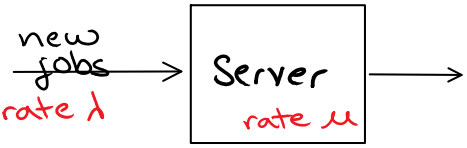
\includegraphics[width=0.3\linewidth, center]{image/queue.png}
            \end{figure}
                \begin{itemize}
                    \item Stationary Distribution $\pi: \pi_i = (1-\frac{\lambda}{\mu})(\frac{\lambda}{\mu})^i$
                    \item For queue with feedback: find the stationary increment frequency $\lambda$ and process frequency $\mu$ then stationary distribution is $\pi: \pi_i = (1-\frac{\lambda}{\mu})(\frac{\lambda}{\mu})^i$
                \end{itemize}
        \end{itemize}
\end{itemize}

\section{Martingales}
\begin{itemize}
    \item Definition
        \begin{itemize}
            \item Discrete

                General Discrete Martingales
                \begin{itemize}
                    \item $\{Z_i\}_{i=0}^\infty$ such that
                        \begin{enumerate}
                            \item $\mathbb{E}[|Z_n|] < \infty$
                            \item $\mathbb{E}[Z_{n+1}| Z_0, \dots, Z_n] = Z_n$
                        \end{enumerate}
                        \begin{itemize}
                            \item sub-martingales: $\mathbb{E}[Z_{n+1}| Z_0, \dots, Z_n] \geq Z_n$
                            \item super-martingales: $\mathbb{E}[Z_{n+1}| Z_0, \dots, Z_n] \leq Z_n$
                        \end{itemize}
                \end{itemize}
                Discrete Martingales with respect to $X_i$
                \begin{itemize}
                    \item $\{Z_i\}_{i=0}^\infty$ such that
                        \begin{enumerate}
                            \item $\mathbb{E}[|Z_n|] < \infty$
                            \item $\mathbb{E}[Z_{n+1}| X_0, \dots, X_n] = Z_n$
                        \end{enumerate}
                        \begin{itemize}
                            \item sub-martingales: $\mathbb{E}[Z_{n+1}| X_0, \dots, X_n] \geq Z_n$
                            \item super-martingales: $\mathbb{E}[Z_{n+1}| X_0, \dots, X_n] \leq Z_n$
                        \end{itemize}
                    \item $\mathbb{E}[Z_{n+1}| X_0, \dots, X_n] = Z_n$ implies $\mathbb{E}[Z_{n+1}| Z_0, \dots, Z_n] = Z_n$
                        \begin{itemize}
                            \item $Z_n$ is a function of $X_0, \dots, X_n$
                            \item $\mathbb{E}[Z_{n+1}| Z_0, \dots, Z_n]$
                                $= \mathbb{E}[\mathbb{E}[Z_{n+1}| X_0, \dots, X_n, Z_0, \dots, Z_n]| Z_0, \dots, Z_n]$

                                $= \mathbb{E}[\mathbb{E}[Z_{n+1}| X_0, \dots, X_n]| Z_0, \dots, Z_n]$
                                $= \mathbb{E}[Z_n| Z_0, \dots, Z_n] = Z_n$
                        \end{itemize}
                \end{itemize}
            \item Continuous Martingales with respect to $N(t)$
                \begin{itemize}
                    \item $Y(t)$ such that
                        \begin{enumerate}
                            \item $\mathbb{E}[|Y(t)|] < \infty$
                            \item $\mathbb{E}[Y(t)| \{N(s) | 0 \leq s \leq \tau\}] = Y(\tau), \forall \tau \leq t$
                        \end{enumerate}
                        \begin{itemize}
                            \item sub-martingales: $\mathbb{E}[Y(t)| \{N(s) | 0 \leq s \leq \tau\}] \geq Y(\tau), \forall \tau \leq t$
                            \item super-martingales: $\mathbb{E}[Y(t)| \{N(s) | 0 \leq s \leq \tau\}] \leq Y(\tau), \forall \tau \leq t$
                        \end{itemize}
                \end{itemize}
        \end{itemize}
    \item Property
        \begin{itemize}
            \item $\mathbb{E}[Z_n] = \mathbb{E}[Z_1]$

                Proof: $\mathbb{E}[Z_{n+1} - Z_n] = \mathbb{E}[\mathbb{E}[Z_{n+1} - Z_n| Z_0, \dots, Z_n]] = 0$
            \item $\mathbb{E}[Z_n | \{Z_i | i \in S\}] = Z_{\max_{i \in S} i}$, where $\forall i \in S, i < n$

                Proof: $\mathbb{E}[Z_n| Z_i] = \mathbb{E}[\mathbb{E}[Z_n| Z_0, \dots, Z_{n-1}]|Z_i] = \mathbb{E}[Z_{n-1}| Z_i]$
            \item Azuma's Inequality
                \begin{itemize}
                    \item $\mu = \mathbb{E}[Z_0]$
                    \item $-a_i \leq Z_i - Z_{i-1} \leq b_i$
                    \item $P[|Z_n - \mu| \geq \delta] \leq 2 e^{- \frac{2\delta^2}{\sum_{i=1}^n(b_i + a_i)^2}}$
                \end{itemize}
            \item Kolmogorov's sub-martingales inequality
                \begin{itemize}
                    \item $P[\sup_{n \geq 1}Z_n \geq a] \leq \frac{\mathbb{E}[Z_1]}{a}$
                \end{itemize}
            \item Martingales Stopping Theorem
                \begin{itemize}
                    \item Stopping Times: a random variable $\tau$ s.t. $\{\tau = n\}$ is independent of $\{X_i\}_{i=n+1}^\infty$
                    \item Stopping Condition: a condition to stop if we can consider $\tau = \min\{n: \text{ condition}(n) = \top \}$
                    \item $\mathbb{E}[Z_\tau] = \mathbb{E}[Z_0]$ if the either of the following holds
                        \begin{enumerate}
                            \item $P[\tau \leq k] = 1$
                            \item $P[\max_{i \leq \tau} |Z_\tau| \leq k] = 1$ 
                            \item $\mathbb{E}[\tau] < k$ and $\mathbb{E}[|Z_{n+1} - Z_n|| Z_0, \dots, Z_n] < k$
                        \end{enumerate}
                \end{itemize}
        \end{itemize}
    \item Application for generating Martingales
        \begin{itemize}
            \item Sum of iid. random variables
                \begin{itemize}
                    \item $\{X_i\}_{i=1}^\infty$ are iid. random variables
                    \item $Z_n = \sum_{i=1}^n X_i - n \mathbb{E}[X_i]$ is a martingales.
                    \item Proof: $\mathbb{E}[Z_{n+1}| Z_0, \dots, Z_n]$
                        $= \mathbb{E}[Z_n + X_{n+1} - \mathbb{E}[X_i]| Z_0, \dots, Z_n] = Z_n$
                \end{itemize}
            \item Squre of sum of iid. random variables
                \begin{itemize}
                    \item $\{X_i\}_{i=1}^\infty$ are iid. random variables and $\mathbb{E}[X_i] = 0$
                    \item $Z_n = (\sum_{i=1}^n X_i)^2 - n \mathbb{E}[X_i^2]$ is a martingales.
                    \item Proof: $\mathbb{E}[Z_{n+1}| Z_0, \dots, Z_n]$
                        $= \mathbb{E}[Z_n + X_{n+1}^2 + 2X_{n+1}(\sum_{i=1}^n X_i) - \mathbb{E}[X_i^2]| Z_0, \dots, Z_n] = Z_n$
                \end{itemize}
            \item Product of iid. random variables
                \begin{itemize}
                    \item $\{X_i\}_{i=1}^\infty$ are iid. random variables
                    \item $Z_n = \frac{\prod_{i=1}^n X_i}{\mathbb{E}[X_i]^n}$ is a martingales.
                    \item Proof: $\mathbb{E}[Z_{n+1}| Z_0, \dots, Z_n]$
                        $= \mathbb{E}[Z_n(\frac{X_{n+1}}{\mathbb{E}[X_i]})| Z_0, \dots, Z_n] = Z_n$
                \end{itemize}
            \item Poisson Process
                \begin{itemize}
                    \item $N(t)$ is a poisson process
                    \item $Y(t) = N(t) - \lambda t$ is a martingales.
                    \item Proof: $\mathbb{E}[Y(t)| \{N(s) | 0 \leq s \leq \tau\}]$
                        $= \mathbb{E}[Y(\tau) + Y(t) - Y(\tau)| \{N(s) | 0 \leq s \leq \tau\}]$

                        $= Y(\tau) + \mathbb{E}[N(t) - N(\tau) + \lambda(t - \tau)| \{N(s) | 0 \leq s \leq \tau\}] = Y(\tau)$
                \end{itemize}
            \item Doob-type Martingales
                \begin{itemize}
                    \item $X, \{Y_i\}_{i=1}^\infty$ are random variables
                    \item $Z_n = \mathbb{E}[X|Y_1, Y_2, \dots, Y_n]$ is a martingales
                    \item Proof: $\mathbb{E}[Z_{n+1}| Y_1, \dots, Y_n]$
                        $= \mathbb{E}[\mathbb{E}[X|Y_1, Y_2, \dots, Y_n, Y_{n+1}]| Y_1, Y_2, \dots, Y_n]$

                        $= \mathbb{E}[X| Y_1, Y_2, \dots, Y_n] = Z_n$
                \end{itemize}
        \end{itemize}
    \item Example
        \begin{itemize}
            \item Symmetric Random Walk
                \begin{itemize}
                    \item $p = 0.5$
                    \item $\tau = \min\{i|\sum_{i=0}^n X_i \in \{-a, b\}\}$
                    \item $Z_n = \sum_{i=0}^n X_i$, by second rule of Martingales Stopping Theorem: $\mathbb{E}[Z_\tau] = 0$

                        $\rightarrow P[Z_\tau \text{ at }a ] = \frac{b}{a+b}, P[Z_\tau \text{ at }b ] = \frac{a}{a+b}$
                    \item $Z_n = (\sum_{i=0}^n X_i)^2 - n$, by third rule of Martingales Stopping Theorem: $\mathbb{E}[Z_\tau] = 0$

                        $\rightarrow \mathbb{E}[\tau] = ab$
                \end{itemize}
            \item Unbiased Random Walk
                \begin{itemize}
                    \item $\tau = \min\{i|\sum_{i=0}^n X_i \in \{-a, b\}\}$
                    \item $Z_n = (\frac{1-p}{p})^{\sum_{i=0}^n X_i}$, by second rule of Martingales Stopping Theorem: $\mathbb{E}[Z_\tau] = 0$

                        $P[Z_\tau \text{ at }a ] = \frac{(\frac{1-p}{p})^{b}-1}{(\frac{1-p}{p})^b - (\frac{1-p}{p})^{-a}}, P[Z_\tau \text{ at }b ] = \frac{1-(\frac{1-p}{p})^{-a}}{(\frac{1-p}{p})^b - (\frac{1-p}{p})^{-a}}$
                    \item $Z_n = \sum_{i=0}^n X_i - n \mathbb{E}[X_0]$, by third rule of Martingales Stopping Theorem: $\mathbb{E}[Z_\tau] = 0$

                        $\rightarrow \mathbb{E}[\tau] = \frac{\mathbb{E}[\sum_{i=0}^\tau X_i]}{\mathbb{E}[X_0]}$
                \end{itemize}
        \end{itemize}
\end{itemize}

\section{Random Walk}
\begin{itemize}
    \item Definition
        \begin{itemize}
            \item $X_i = \left\{ \begin{array}{ll}
                        1 & \text{with probability } p \\ 
                        -1 & \text{with probability } 1-p \\ 
                    \end{array} \right.$
            \item $S_n = \sum_{i = 0}^n X_i$
        \end{itemize}
    \item The monkey at the cliff
        \begin{itemize}
            \item $P_k = P[ \exists n \text{ such that } S_n = k] = \left\{ \begin{array}{cc}
                1 & \text{if } p \geq \frac{1}{2} \\
                (\frac{p}{1-p})^k & \text{if } p < \frac{1}{2} \\
                \end{array} \right.$ where $k \in \mathbb{N}$

                Proof
                \begin{itemize}
                    \item $P_k = P_1^k$ by memoryless property
                    \item $P_1 = p + q \times P_2 \rightarrow P_1 = 1$ or $\frac{p}{1-p}$
                    \item if $p \geq 0.5 \rightarrow P_1 = 1$ ($P_1 \leq 1$)
                    \item if $p < 0.5 \rightarrow P_1 = \frac{p}{1-p}$

                        Since $P_1 \leq \frac{p}{1-p}$ by induction on $n$ to $\infty$ for $P_1(n) = P[S_n = k]$
                \end{itemize}
            \item $\mathbb{E}_k = \mathbb{E}[\min\{n:S_n =k\}] = \left\{ \begin{array}{cc}
                \infty & \text{if } p \leq \frac{1}{2} \\
                \frac{k}{2p-1} & \text{if } p > \frac{1}{2} \\
                \end{array} \right.$ where $k \in \mathbb{N}$

                Proof
                \begin{itemize}
                    \item $\mathbb{E}_k = \mathbb{E}_1 \times k$ by memoryless property
                    \item $\mathbb{E}_1 = 1 + 0 \times p + \mathbb{E}_2 \times (1-p)$
                    \item if $p < 0.5 \rightarrow P_1 = \frac{p}{1-p} \rightarrow \mathbb{E}_1 = \infty$
                    \item if $p = 0.5 \rightarrow \mathbb{E}_1 = 1 + \mathbb{E}_1$ (no solution) $\rightarrow \mathbb{E}_1 = \infty$
                    \item if $p > 0.5 \rightarrow \mathbb{E}_1 = \frac{1}{2p-1}$
                \end{itemize}
            \item $P_0 = P[ \exists n \text{ such that } S_n = 0] = 1 - |2p-1|$ where $k \in \mathbb{N}$
                \begin{itemize}
                    \item $P_0 = p \times P_{-1} + (1-p) \times P_1$
                \end{itemize}
            \item $\mathbb{E}_0 = \mathbb{E}[\min\{n:S_n =0\}] = \infty$
                \begin{itemize}
                    \item if $p \not = \frac{1}{2} \rightarrow P_0 \not = 1 \rightarrow \mathbb{E}_0 = \infty$
                    \item if $p = \frac{1}{2} \rightarrow \mathbb{E}_0 = 1 + \frac{1}{2} \mathbb{E}_{-1} + \frac{1}{2} \mathbb{E}_1 = \infty$
                \end{itemize}
        \end{itemize}
    \item The Gambler's Ruin
        \begin{itemize}
            \item Definition: $\tau = \min\{i| S_n \in \{-a, b\}\}$
            \item $A_k = P[S_\tau = b | X_0 = k]$
                \begin{itemize}
                    \item $A_k = p A_{k+1} + (1-p) A_{k-1}$
                \end{itemize}
            \item $A_0 = \left\{ \begin{array}{cc}
                        \frac{a}{a+b} & \text{if } p = \frac{1}{2} \\
                        \frac{(\frac{1-p}{p})^a - 1}{(\frac{1-p}{p})^{a+b} - 1} & \text{if } p \not = \frac{1}{2} \\
                \end{array} \right.$

                Solved by previous recursive equation
            \item $E_k = \mathbb{E}[\tau|X_0 = k]$
                \begin{itemize}
                    \item $E_k = 1 + p E_{k+1} + (1-p) E_{k-1}$
                \end{itemize}
            \item $E_0 = \left\{ \begin{array}{cc}
                        ab & \text{if } p = \frac{1}{2} \\
                        \frac{a}{1-2p} - \frac{a+b}{1-2p} \times \frac{(\frac{1-p}{p})^a - 1}{(\frac{1-p}{p})^{a+b} - 1} & \text{if } p \not = \frac{1}{2} \\
                \end{array} \right.$

                Solved by previous recursive equation
        \end{itemize}
    \item Observation
        \begin{itemize}
            \item $S_n = O(n)$

                Upperbound: $\lim_{n \rightarrow \infty} P[S_n \leq k\sqrt{n}] = \int_{-\infty}^k \frac{1}{2 \pi} e^{-\frac{x^2}{2}} dx$

                Lowerbound: $P[|S_n| \geq k\sqrt{n}] \leq 2 e^{-\frac{k^2}{2}}$
        \end{itemize}
\end{itemize}

\section{Brownian Motion}
\begin{itemize}
    \item Standard Brownian Motion
        \begin{itemize}
            \item Interpretation: generalize discrete time and space of random walk to be in continuous time and space
                \begin{itemize}
                    \item $S_t = \delta_x (\sum_{i=0}^{\frac{t}{\delta_t}} X_i)$
                    \item let $\delta_x = \sqrt{\delta_t}$ and $\delta_x \rightarrow 0$
                    \item $\mathbb{E}[S_t] = 0$
                    \item $\mathit{Var}(S_t) = t$
                        \begin{itemize}
                            \item $\mathit{Var}(S_t) = \delta_x^2 \frac{t}{\delta_t} = t$
                        \end{itemize}
                \end{itemize}
            \item Definition:
                \begin{itemize}
                    \item $X(0) = 0$
                    \item $X(t) \sim N(0, \sigma^2 = t)$
                    \item $X(t)$ has independent, stationary increment
                        \begin{itemize}
                            \item independent: $X(t_{i_2}) - X(t_{i_1})$ and $X(t_{i_1}) - X(t_{i_0})$ are independent
                            \item stationary: $X(s + t) - X(t) = X(s)$
                        \end{itemize}
                \end{itemize}
            \item Property
                \begin{itemize}
                    \item Distribution self-similarity
                        \begin{itemize}
                            \item $X(t) \sim N(0, t)$
                            \item $\sqrt{k}X(\frac{t}{k}) \sim N(0, t)$
                        \end{itemize}
                    \item Nowhere Differentiable
                        \begin{itemize}
                            \item With probability 1, $X(t)$ is nowhere differentiable
                            \item $\lim_{\delta_t \rightarrow 0} \frac{X(t+\delta_t) - X(t)}{\delta_t} = \lim_{\delta_t \rightarrow 0} \frac{N(0, \delta_t}{\delta_t} = \lim_{\delta_t \rightarrow 0} N(0, \frac{1}{\delta_t})$
                        \end{itemize}
                    \item Unbounded Variation
                        \begin{itemize}
                            \item Length of distance $\rightarrow \infty$ in finite time $t$
                            \item $\lim_{n \rightarrow \infty} \sum_{j=1}^n |X(\frac{jt}{n}) - X(\frac{(j-1)t}{n})| = \infty$

                                Proof: $\lim_{n \rightarrow \infty} \sum_{j=1}^n |X(\frac{jt}{n}) - X(\frac{(j-1)t}{n})|$
                                $= lim_{n \rightarrow \infty} \sum_{j=1}^n |X(\frac{t}{n})| = n \times \sqrt{\frac{2}{\pi} \frac{t}{n}} = \infty$
                        \end{itemize}
                    \item Hitting Time

                            The Gambler's Ruin
                            \begin{itemize}
                                \item $\tau = \min\{t \geq 0: X(t) \in \{-A, B\}\}$
                                \item $P[X(\tau) = A] = \frac{B}{A+B}, P[X(\tau) = B] = \frac{A}{A+B}$

                                    Prove by Martingales Stopping Theorem on $X(t)$:

                                    $\rightarrow \mathbb{E}[X(t)] = P[X(\tau) = A]A + P[X(\tau) = B]B = 0$
                                \item $\mathbb{E}[\tau] = AB$

                                    Prove by Martingales Stopping Theorem on $X(t)^2 - t$:

                                    $\rightarrow \mathbb{E}[X(t)^2 - t] = P[X(\tau) = A]A^2 + P[X(\tau) = B]B^2 - \mathbb{E}[\tau] = 0$
                            \end{itemize}
                            The monkey at the cliff
                            \begin{itemize}
                                \item $\tau = \min\{t \geq 0: X(t) = B\}$
                                \item $P[\tau < \infty] = 1$

                                    Prove by let $A = -\infty$ in The Gambler's Ruin
                                \item $P[\tau \leq t] = 2 P[X(\tau) \geq B]$

                                    $P[\tau \leq t] = P[\tau \leq t \text{ and } X(t) \geq B] + P[\tau \leq t \text{ and } X(t) < B]$

                                    $= 2 P[\tau \leq t \text{ and } X(t) \geq B]$
                                    $= 2 P[X(t) \geq B]$
                                \item $\mathbb{E}[\tau] = \infty$

                                    Prove by let $A = -\infty$ in The Gambler's Ruin
                            \end{itemize}
                    \item Diffusion Equation
                        \begin{itemize}
                            \item Forward Diffusion Equation: $\frac{\partial f}{\partial t} = \frac{1}{2} \frac{\partial^2 f}{\partial x^2}$
                            \item Backward Diffusion Equation: $\frac{\partial f}{\partial t} = \frac{-1}{2} \frac{\partial^2 f}{\partial x^2}$
                            \item $f(X(t_2) = x| X(t_1) = k)$ satisfies Forward Diffusion equation
                            \item $f(X(t_2) = k| X(t_1) = x)$ satisfies Backward Diffusion equation
                        \end{itemize}
                    \item Martingales
                        \begin{itemize}
                            \item $X(t)$ is a martingale
                            \item $X(t)^2 - t$ is a martingale
                            \item $e^{cX(t) - \frac{c^2}{2}t}$ is a martingale
                        \end{itemize}
                    \item Zeros

                        Definition: $P[X(t) = 0, t_0 < t < t_1] = \frac{2}{\pi} \cos^{-1}(\sqrt{\frac{t_0}{t_1}})$
                        \begin{itemize}
                            \item Prove by $P[X(t) = 0, t_0 < t < t_1] = \int_{-\infty}^{\infty} f_{X(t_0}(x_1) P[T_{-x} \leq t_1 - t_0] dx_1$
                        \end{itemize}
                        Property
                        \begin{itemize}
                            \item $P[X(t) = 0, 0 < t < t_1] = 1, \forall t_1 > 0$
                            \item $P[\mathit{inf}\{t > 0: X(t)=0\} = 0] = 1$
                            \item $P[\text{ there are infinitely many zeros in }[0, t]] = 1$
                        \end{itemize}
                \end{itemize}
            \item Brownian Bridge
                \begin{itemize}
                    \item Definition: the distribution of $t_1$ given the result of the future $X(t_2)$
                    \item Property


                        $f_{X(t_1)|X(t_2)}(x_1, x_2) = \frac{f_{X(t_1), X(t_2)}(x_1, x_2)}{f_{X(t_2)}(x_2)} \sim N(\frac{t_1}{t_2}x_2, \frac{t_1(t_2 - t_1)}{t_2})$
                        \begin{itemize}
                            \item let $s = t_2 - t_1$
                            \item $f_{X(t_1)|X(t_2)}(x_1, x_2) = \frac{f_{X(t_1), X(t_2)}(x_1, x_2)}{f_{X(t_2)}(x_2)}$

                                $= \frac{f_{X(t_1), X(s)}(x_1, x_2 - x_1)}{f_{X(t_2)}(x_2)}$ (By transformation of 2-D random variables)

                                $= \frac{f_{X(t_1)}(x_1) f_{X(s)}(x_2 - x_1)}{f_{X(t_2)}(x_2)}$
                                $= \frac{\frac{1}{\sqrt{2\pi t_1}}e^{\frac{-x_1^2}{2t_1}} \frac{1}{\sqrt{2\pi(t_2 - t_1)}}e^{\frac{-(x_2-x_1)^2}{2(t_2 - t_1)}}}{\frac{1}{\sqrt{2\pi t_2}}e^{\frac{-x_2^2}{2t_2}}}$

                                $= \frac{1}{\sqrt{2\pi \frac{t_1(t_2 - t_1)}{t_2}}}e^{\frac{-(x_1 - \frac{t_1}{t_2}x_2)^2}{2\frac{t_1(t_2 - t_1)}{t_2}}} \rightarrow X(t_1) - \frac{t_1}{t_2}X(t_2) \sim N(0, \frac{t_1(t_2 - t_1)}{t_2})$
                            \item $\mathbb{E}[X(t_1)|X(t_2)] = \frac{t_1}{t_2}X(t_2)$
                            \item $\mathit{Var}(X(t_1)|X(t_2)) = \frac{t_1(t_2 - t_1)}{t_2}$
                            \item $Y(t_1) = X(t_1) - \frac{t_1}{t_2} X(t_2)$ share the same distribution as $X(t_1) |X(t_2) = 0$
                        \end{itemize}
                        $\mathit{Cov}(X(t_1), X(t_2)|X(t_3)) = \frac{t_1(t_3-t_2)}{t_3}$
                        \begin{itemize}
                            \item $\mathit{Cov}(X(t_1), X(t_2)|X(t_3))$

                                $= \mathbb{E}[X(t_1)X(t_2)|X(t_3)] - \mathbb{E}[X(t_1)|X(t_3)] \times \mathbb{E}[X(t_2)|X(t_3)]$

                                $= \mathbb{E}[X(t_1)^2 + X(t_1)(X(t_2)-X(t_1))|X(t_3)] - \frac{t_1 t_2}{t_3^2} X(t_3)^2$
                                % $= \frac{t_1^2}{t_3^2}X(t_3)^2 + \frac{t_1(t_3- t_1)}{t_3} + \mathbb{E}[X(t_1)(X(t_2)-X(t_1))|X(t_3)] - \frac{t_1 t_2}{t_3^2} X(t_3)^2$

                                $= \mathbb{E}[X(t_1)(X(t_2)-X(t_1))|X(t_3)] + \frac{t_1 (t_1 - t_2)}{t_3^2} X(t_3)^2 + \frac{t_1(t_3- t_1)}{t_3}$

                                {\tiny
                                $= \int_{-\infty}^{\infty} \frac{1}{\sqrt{2\pi \frac{t_1(t_3 - t_1)}{t_3}}}e^{\frac{-(x_1 - \frac{t_1}{t_3}X(3))^2}{2\frac{t_1(t_3 - t_1)}{t_3}}} \mathbb{E}[x_1(X(t_2)-x_1)|X(t_3), X(t_1) = x_1] dx_1 + \frac{t_1 (t_1 - t_2)}{t_3^2} X(t_3)^2 + \frac{t_1(t_3- t_1)}{t_3}$
                                }

                                $= \int_{-\infty}^{\infty} \frac{1}{\sqrt{2\pi \frac{t_1(t_3 - t_1)}{t_3}}}e^{\frac{-(x_1 - \frac{t_1}{t_3}X(3))^2}{2\frac{t_1(t_3 - t_1)}{t_3}}} x_1(-x_1 + X(3))\frac{t_2-t_1}{t_3-t_1} dx_1 + \frac{t_1 (t_1 - t_2)}{t_3^2} X(t_3)^2 + \frac{t_1(t_3- t_1)}{t_3}$

                                $= \frac{t_1(t_2 - t_1)}{t_3^2}X(t_3)^2 - \frac{t_1(t_2-t_1)}{t_3} + \frac{t_1 (t_1 - t_2)}{t_3^2} X(t_3)^2 + \frac{t_1(t_3- t_1)}{t_3}$


                                $= \frac{t_1(t_3-t_2)}{t_3}$
                        \end{itemize}
                \end{itemize}
        \end{itemize}
    \item Brownian Motion with drift
        \begin{itemize}
            \item Interpretation: generalize discrete time and space of biased random walk to be in continuous time and space
                \begin{itemize}
                    \item $X_i = \left\{ \begin{array}{ll}
                                1 & \text{with probability } p \\ 
                                -1 & \text{with probability } 1-p \\ 
                            \end{array} \right.$
                    \item $S_t = \delta_x (\sum_{i=0}^{\frac{t}{\delta_t}} X_i)$
                    \item let $\delta_x = \sqrt{\delta_t}$, $p = \frac{1 + \mu \sqrt{\delta_t}}{2}$, and $\delta_x \rightarrow 0$
                    \item $\mathbb{E}[S_t] = \mu t$
                        \begin{itemize}
                            \item $\mathbb{E}[S_t] = \delta_x \frac{t}{\delta_t} (2p-1) = \mu t$
                        \end{itemize}
                    \item $\mathit{Var}(S_t) = t$
                        \begin{itemize}
                            \item $\mathit{Var}(S_t) = \delta_x^2 \frac{t}{\delta_t} (1-(2p-1)^2) = t$
                        \end{itemize}
                \end{itemize}
            \item Definition:
                \begin{itemize}
                    \item $X(t)$ is Standard Brownian Motion
                    \item $Y(t) = X(t) + \mu t$
                \end{itemize}
            \item Property
                \begin{itemize}
                    \item Hitting Time

                            The Gambler's Ruin
                            \begin{itemize}
                                \item $\tau = \min\{t \geq 0: Y(t) \in \{-A, B\}\}$
                                \item $P[Y(t) = A ] = \frac{e^{-2\mu B} - 1}{e^{-2\mu B} - e^{2\mu A}}, P[Y(t) = B ] = \frac{1-e^{2\mu A}}{e^{-2\mu B} - e^{2\mu A}}$

                                    Prove by Martingales Stopping Theorem on $e^{cX(t) - \frac{c^2}{2}t}$ and $c = -2\mu$:

                                    $\rightarrow \mathbb{E}[e^{c X(t) - \frac{c^2}{2}t}] = \mathbb{E}[e^{-2\mu Y(t)}] = 1$

                                \item $\mathbb{E}[\tau] = \frac{1}{\mu}(P[Y(t) = B] \times (A + B) - A)$

                                    Prove by Martingales Stopping Theorem on $X(t)$:

                                    $\rightarrow \mathbb{E}[X(t)] = P[Y(t) = B] \mathbb{E}[B- \mu t|Y(t) = B] + P[Y(t) = A] \mathbb{E}[- A - \mu t|Y(t) = A] = 0$
                            \end{itemize}
                            The monkey at the cliff
                            \begin{itemize}
                                \item $\tau = \min\{t \geq 0: X(t) = B\}$
                                \item $P[\tau < \infty] = \left\{ \begin{array}{cc}
                                            e^{2\mu B} & \text{if } \mu < 0 \\ 
                                            1 & \text{if } \mu \geq 0 \\ 
                                \end{array}\right.$

                                    Prove by let $A = -\infty$ in The Gambler's Ruin
                            \end{itemize}
                \end{itemize}
        \end{itemize}
    \item Gaussian Process
        \begin{itemize}
            \item Definition: A stochastic process $\{X(t): t \geq 0\}$ such that for every $\{t_i\}_{i=1}^n, [X(t_1), X(t_2), \dots, X(t_n)]$ is a joint Gaussian distribution
                \begin{itemize}
                    \item Defined by
                        \begin{itemize}
                            \item $\mathbb{E}[X(t)], \forall t$
                            \item $\mathit{Cov}(X(s), X(t)), \forall s, t$
                        \end{itemize}
                \end{itemize}
            \item Property
                \begin{itemize}
                    \item Standard Brownian Motion is a Gaussian Process with $\mathbb{E}[X(t)] = 0, \mathit{Cov}(X(s), X(t)) = \min\{s, t\}$
                        \begin{itemize}
                            \item $\mathit{Cov}(X(s), X(t)) = \min(s, t)$ (by $X(t) = X(s) + X(t-s)$ if $t > s$)
                        \end{itemize}
                \end{itemize}
        \end{itemize}
    \item Geometric Brownian Motion
        \begin{itemize}
            \item Definition:
                \begin{itemize}
                    \item $Y(t) = e^{\sigma X(t)}$
                \end{itemize}
            \item Property:
                \begin{itemize}
                    \item $\mathbb{E}[Y(t)] = e^{\frac{\sigma^2 t}{2}}$
                    \item $\mathit{Var}[Y(t)] = e^{\sigma^2 t}$
                \end{itemize}
        \end{itemize}
    \item Brownian Motion reflected at the origin
        \begin{itemize}
            \item Definition:
                \begin{itemize}
                    \item $Z(t) = |X(t)|$
                \end{itemize}
            \item Property
                \begin{itemize}
                    \item $P[Z(t) \geq x] = \frac{2}{\sqrt{2 \pi t}} e^{\frac{-x^2}{2t}}$
                        \begin{itemize}
                            \item same distribution as Maximum Brownian Motion
                        \end{itemize}
                \end{itemize}
        \end{itemize}
    \item Maximum Brownian Motion
        \begin{itemize}
            \item Definition:
                \begin{itemize}
                    \item $Z(t) = \max_{0 \leq s \leq t} X(t)$
                \end{itemize}
            \item Property
                \begin{itemize}
                    \item $P[Z(t) \geq x] = \frac{2}{\sqrt{2 \pi t}} e^{\frac{-x^2}{2t}}$
                        \begin{itemize}
                            \item $P[Z(t) \geq x] = P[T_x \leq t] = \frac{2}{\sqrt{2 \pi t}} e^{\frac{-x^2}{2t}}$
                            \item same distribution as Brownian Motion reflected at the origin
                        \end{itemize}
                \end{itemize}
        \end{itemize}
    \item Tricks
        \begin{itemize}
            \item Creat $Y_1, Y_2 \sim N(0, 1)$ and $\mathit{Cov}(Y_1, Y_2) = \cos \theta$
                \begin{itemize}
                    \item $X_1, X_2 \sim N(0, 1)$ and independent
                    \item $Y_1 = X_1$
                    \item $Y_2 = \cos \theta \times X_1 + \sin \theta \times X_2$
                \end{itemize}
        \end{itemize}
\end{itemize}

\section{Stochastic Calculus}
\begin{itemize}
    \item Mischellany
        \begin{itemize}
            \item $\lim_{n \rightarrow \infty} \sum_{i=1}^n (B(\frac{i-1}{n}t) - B(\frac{i}{n}t))^2$ converge to $t$ in mean square

                Proof
                \begin{itemize}
                    \item $\mathbb{E}[\lim_{n \rightarrow \infty} \sum_{i=1}^n (B(\frac{i-1}{n}t) - B(\frac{i}{n}t))^2] = t$
                    \item $\mathit{Var}(\lim_{n \rightarrow \infty} \sum_{i=1}^n (B(\frac{i-1}{n}t) - B(\frac{i}{n}t))^2) = 0$

                    $\mathit{Var}(\lim_{n \rightarrow \infty} \sum_{i=1}^n (B(\frac{i-1}{n}t) - B(\frac{i}{n}t))^2)$
                    $= \lim_{n \rightarrow \infty} \sum_{i=1}^n \mathit{Var}((B(\frac{i-1}{n}t) - B(\frac{i}{n}t))^2)$

                    $= \lim_{n \rightarrow \infty} \sum_{i=1}^n 2 \frac{t}{n}^2 = \frac{t^2}{n} = 0$
                \end{itemize}
        \end{itemize}
    \item Given a continuous function $f(x)$, $g(x, B(x))$, and a standard Brownian motion $B(x)$
    \item $\int_{x=0}^t f(x) dB(x)$

        Definition
        \begin{itemize}
            \item $\int_{x=0}^t f(x) dB(x) = \lim_{n \rightarrow \infty} \sum_{i=1}^n f(\frac{i}{n}t)(B(\frac{i}{n}t) - B(\frac{i-1}{n}t))$
        \end{itemize}
        Property
        \begin{itemize}
            \item $\int_{x=0}^t f(x) dB(x)$ exists (limit converges)
            \item The integral is normally distributed

                Proof:
                \begin{itemize}
                    \item the integral is the sum of independent Gaussian random variable
                \end{itemize}
            \item $\mathbb{E}[\int_{x=0}^t f(x) dB(x)] = 0$
            \item $\mathit{Var}[\int_{x=0}^t f(x) dB(x)] = \int_0^t f(x)^2 dx$

                Proof:
                \begin{itemize}
                    \item $\mathit{Var}(\int_{x=0}^t f(t) dB(t)) = \lim_{n \rightarrow \infty} \sum_{i=1}^n \mathit{Var}(f(\frac{i}{n}t)(B(\frac{i}{n}t) - B(\frac{i-1}{n}t)))$

                        $= \lim_{n \rightarrow \infty} \sum_{i=1}^n f(\frac{i}{n}t)^2 \frac{i}{n} = \int_0^t f(x)^2 dx$
                \end{itemize}
            \item $\int_{x=0}^{t_1} f(x) dB(x)$ and $\int_{x=0}^{t_2} g(x) dB(x)$ are jointly normal and

                $\mathit{Cov}(\int_{x=0}^{t_1} f(x) dB(x), \int_{x=0}^{t_2} g(x) dB(x) = \int_0^{\min\{t_1, t_2\}} f(x)g(x) dx$

                Proof:
                \begin{itemize}
                    \item Suppose $t = \min\{t_1, t_2\}$
                    \item $\mathit{Cov}(\int_{x=0}^{t_1} f(x) dB(x), \int_{x=0}^{t_2} g(x) dB(x))$

                        $= \lim_{n \rightarrow \infty} \sum_{i=1}^n \mathit{Cov}(f(\frac{i}{n}t)(B(\frac{i}{n}t) - B(\frac{i-1}{n}t)), g(\frac{i}{n}t)(B(\frac{i}{n}t) - B(\frac{i-1}{n}t)))$

                        $= \lim_{n \rightarrow \infty} \sum_{i=1}^n f(\frac{i}{n}t)g(\frac{i}{n}t) \frac{i}{n} = \int_0^t f(x)g(x) dx$
                \end{itemize}
        \end{itemize}
    \item $\int_{x=0}^t f'(x) B(x) dx$

        Definition
        \begin{itemize}
            \item $\int_{x = 0}^t f'(x) B(x) dx = [f(x) B(x)]_{x=0}^t - \int_{x = 0}^t f(x) dB(x)$

                Proof:
                \begin{itemize}
                    \item Use integration by part to integrate over $B(x)$
                    \item $[f(x) B(x)]_{x=0}^t = \int_{x = 0}^t f(x) dB(x) + \int_{x = 0}^t B(x) df(x)$
                \end{itemize}
        \end{itemize}
        Example
        \begin{itemize}
            \item $\int_{x = 0}^t B(x) dx = B(t)t - \int_{x=0}^t x dB(x) = \int_{x=0}^t (t-x) dB(x)$
        \end{itemize}
    \item $\int_{x=0}^t g(x, B(x)) dB(x)$

        Definition
        \begin{itemize}
            \item $\tau_j \in [ \frac{i-1}{n}t, \frac{i}{n}t]$
            \item $\int_{x=0}^t g(x, B(x)) dB(x) = \lim_{n \rightarrow \infty} \sum_{i=1}^n g(\tau_j, B(\tau_j))(B(\frac{i}{n}t) - B(\frac{i-1}{n}t))$
            \item Choice of $\tau_j$ will not converge unlike Riemann integral

                check by simulation
        \end{itemize}
        It\^{o} Integral: left endpoint integral
        \begin{itemize}
            \item Definition
                \begin{itemize}
                    \item Condition: $\int_0^t \mathbb{E}[g(x, B(x))]^2 dx < \infty$
                    \item $\tau_j = \frac{i-1}{n}t$
                    \item $\int_{x=0}^t g(x, B(x)) dB(x) = \lim_{n \rightarrow \infty} \sum_{i=1}^n g(\tau_j, B(\tau_j))(B(\frac{i}{n}t) - B(\frac{i-1}{n}t))$
                \end{itemize}
            \item Calculus
                \begin{enumerate}
                    \item By Definition
                    \item By It\^{o}'s Lemma

                        Concept
                        \begin{itemize}
                            \item $(d B(x))^2 = d x$
                                \begin{itemize}
                                    \item By $\lim_{n \rightarrow \infty} \sum_{i=1}^n (B(\frac{i-1}{n}t) - B(\frac{i}{n}t))^2$ converge to $t$ in mean square
                                \end{itemize}
                        \end{itemize}
                        Equation
                        \begin{enumerate}
                            \item $d g(B(x)) = g'(B(x)) d B(x) + \frac{1}{2} g''(B(x)) dx$
                                \begin{itemize}
                                    \item $g(B(x + \delta_x)) - g(B(x)) = g'(B(x)) (B(x+\delta_x) - B(x)) + \frac{1}{2} g''(B(x)) (B(x+\delta_x) - B(x))^2$ (by Taylor series)
                                    \item $g(B(x + \delta_x)) - g(B(x)) = g'(B(x)) (B(x+\delta_x) - B(x)) + \frac{1}{2} g''(B(x)) \delta_x$ (by $(B(x+\delta_x) - B(x))^2$ converges to $\delta_t$)
                                \end{itemize}
                            \item $d g(x, B(x)) = \frac{\partial g(x, B(x))}{\partial B(x)} d B(x) + \frac{\partial g(x, B(x))}{\partial x} d x + \frac{1}{2} \frac{\partial^2 g(x, B(x))}{\partial B(x)^2} d x$
                                \begin{itemize}
                                    \item $g(x + \delta_x, B(x + \delta_x)) - g(x, B(x)) = \frac{\partial g(x, B(x))}{\partial x} d x + \frac{\partial g(x, B(x))}{\partial B(x)} d B(x) + \frac{1}{2} \frac{\partial^2 g(x, B(x))}{\partial x^2} (d x)^2 + \frac{1}{2} \frac{\partial^2 g(x, B(x))}{\partial B(x)^2} (d B(x))^2 + \frac{\partial^2 g(x, B(x))}{\partial x \partial B(x)} d x d B(x)$ (by Taylor series)
                                    \item $g(x + \delta_x, B(x + \delta_x)) - g(x, B(x)) = \frac{\partial g(x, B(x))}{\partial x} d x + \frac{\partial g(x, B(x))}{\partial B(x)} d B(x) + \frac{1}{2} \frac{\partial^2 g(x, B(x))}{\partial B(x)^2} d x$ (by $(B(x+\delta_x) - B(x))^2$ converges to $\delta_t$)
                                \end{itemize}
                            \item $d g(x_1+ \delta_{x_1}, \dots, x_n + \delta_{x_n}) = \sum_{i=1}^n \frac{\partial g(x_1 + \delta_{x_1}, \dots, x_n + \delta_{x_n})}{\partial x_i} d x_i$

                                $+ \frac{1}{2} \sum_{i=1}^n \frac{\partial g(x_1 + \delta_{x_1}, \dots, x_n + \delta_{x_n})}{\partial x_i^2} (d x_i)^2 + \sum_{i < j} \frac{\partial g(x_1 + \delta_{x_1}, \dots, x_n + \delta_{x_n})}{\partial x_i \partial x_j} d x_i d x_j$ (by Taylor series for chain rule)
                        \end{enumerate}
                \end{enumerate}
            \item Property
                \begin{itemize}
                    \item Margingale random variable

                        $\int_{x=0}^t g(x, B(x)) dB(x)$ is a martingale random variable
                        \begin{itemize}
                            \item $\mathbb{E}[g(\frac{i-1}{n}t, B(\frac{i-1}{n}t)) (B(\frac{i}{n}t) - B(\frac{i-1}{n}t))] = 0$ (by independence of $B(\frac{i-1}{n}t)$ and $B(\frac{i}{n}t) - B(\frac{i-1}{n}t)$)
                            \item $\mathbb{E}[\int_{x=0}^{t_2} g(x, B(x)) dB(x)|\int_{x=0}^{t_1} g(x, B(x)) dB(x)]$

                            $= \mathbb{E}[\int_{x=0}^{t_1} g(x, B(x)) dB(x) + \int_{x=t_1}^{t_2} g(x, B(x)) dB(x)|\int_{x=0}^{t_1} g(x, B(x)) dB(x)]$

                            $= \int_{x=0}^{t_1} g(x, B(x)) dB(x) + \mathbb{E}[\int_{x=t_1}^{t_2} g(x, B(x)) dB(x)|\int_{x=0}^{t_1} g(x, B(x)) dB(x)]$

                            $= \int_{x=0}^{t_1} g(x, B(x)) dB(x) + \mathbb{E}[\lim_{n \rightarrow \infty} \sum_{i=1}^n g(\frac{i-1}{n}(t_2-t_1), B(\frac{i-1}{n}(t_2-t_1))) (B(\frac{i}{n}(t_2 - t_1)) - B(\frac{i-1}{n}(t_2 - t_1)))$

                            $= \int_{x=0}^{t_1} g(x, B(x)) dB(x)$
                        \end{itemize}
                        $\mathbb{E}[\int_{x=0}^t g(x, B(x)) dB(x)] = 0$

                        Since Martingales property is more important $\rightarrow$ It\^{o} integral is generally used
                    \item Linear
                        \begin{itemize}
                            \item $\int_{x=0}^t (\alpha g_1(x, B(x)) + \beta g_2(x, B(x)) ) dB(x)$

                                $= \alpha \int_{x=0}^t g_1(x, B(x)) dB(x) + \beta \int_{x=0}^t g_2(x, B(x)) dB(x)$
                        \end{itemize}
                    \item Isometry
                        \begin{itemize}
                            \item $\mathbb{E}[(\int_{x=0}^t g(x, B(x)) dB(x))^2] = \int_0^t \mathbb{E}[(g(x, B(x)) )^2] dx$

                                Proof: $\mathbb{E}[(\int_{x=0}^t g(x, B(x)) dB(x))^2] = \sum_{i=1}^n \mathbb{E}[ g(\frac{i-1}{n}t, B(\frac{i-1}{n}t))^2 (B(\frac{i}{n}t) - B(\frac{i-1}{n}t))^2]$
                        \end{itemize}
                    \item Chain Rule
                        \begin{itemize}
                            \item Given $f(g)$ and $g(x, B(x))$
                            \item Extend $f$ as $d f(x_1+ \delta_{x_1}, \dots, x_n + \delta_{x_n}) = \sum_{i=1}^n \frac{\partial f(x_1 + \delta_{x_1}, \dots, x_n + \delta_{x_n})}{\partial x_i} d x_i$

                                        $+ \frac{1}{2} \sum_{i=1}^n \frac{\partial f(x_1 + \delta_{x_1}, \dots, x_n + \delta_{x_n})}{\partial x_i^2} (d x_i)^2 + \sum_{i < j} \frac{\partial f(x_1 + \delta_{x_1}, \dots, x_n + \delta_{x_n})}{\partial x_i \partial x_j} d x_i d x_j$
                        \end{itemize}
                    \item Product Rule
                        \begin{itemize}
                            \item $d f_1(x, B(x)) = \mu_1(x, B(x)) dx + \sigma_1(x, B(x)) d B(x)$
                            \item $d f_2(x, B(x)) = \mu_2(x, B(x)) dx + \sigma_2(x, B(x)) d B(x)$
                            \item $df_1(x, B(x)) f_2(x, B(x)) = f_2(x, B(x)) df_1(x, B(x)) + f_1(x, B(x)) df_2(x, B(x))$

                                $+ d f_1(x, B(x)) df_2(x, B(x))$
                            \item $df_1(x, B(x)) f_2(x, B(x))$

                                $= f_2(x, B(x)) (\mu_1(x, B(x)) dx + \sigma_1(x, B(x)) d B(x))$

                                $+ f_1(x, B(x)) (\mu_2(x, B(x)) dx + \sigma_2(x, B(x)) d B(x))$

                                $+ \sigma_1(x, B(x))\sigma_2(x, B(x))dx$
                        \end{itemize}
                    \item Quotient Rule
                        \begin{itemize}
                            \item $d f_1(x, B(x)) = \mu_1(x, B(x)) dx + \sigma_1(x, B(x)) d B(x)$
                            \item $d f_2(x, B(x)) = \mu_2(x, B(x)) dx + \sigma_2(x, B(x)) d B(x)$
                            \item $d\frac{1}{f_1(x, B(x))} = - \frac{1}{f_1^2(x, B(x))} df_1(x, B(x)) + \frac{1}{f_1^3(x, B(x))} (df_1(x, B(x)))^2$
                            \item $df_1(x, B(x)) f_2(x, B(x))$ by combining the above three equations
                        \end{itemize}
                \end{itemize}
            \item Example
                \begin{itemize}
                    \item $\int_0^t B(x) d B(x)$
                        \begin{itemize}
                            \item $\int_{x=0}^t B(x) dB(x) = \lim_{n \rightarrow \infty} \sum_{i=1}^n B(\frac{i-1}{n}t) (B(\frac{i}{n}t) - B(\frac{i-1}{n}t))$ (By Definition)

                            $= \lim_{n \rightarrow \infty} \sum_{i=1}^n B(\frac{i-1}{n}t) B(\frac{i}{n}t) - B(\frac{i-1}{n}t)^2$

                            $= \frac{-1}{2} \lim_{n \rightarrow \infty} \sum_{i=1}^n (B(\frac{i-1}{n}t) - B(\frac{i}{n}t))^2 + \frac{B(t)^2}{2}$

                            $= \frac{-1}{2} t + \frac{B(t)^2}{2}$ (By convergence of $\lim_{n \rightarrow \infty} \sum_{i=1}^n (B(\frac{i-1}{n}t) - B(\frac{i}{n}t))^2$)
                        \end{itemize}
                    \item $\int_0^t e^{B(x) - \frac{x}{2}} d B(x)$
                        \begin{itemize}
                            \item $d e^{B(x) - \frac{x}{2}} = e^{B(x) - \frac{x}{2}} d B(x) + \frac{-1}{2} e^{B(x) - \frac{x}{2}} d x + \frac{1}{2} e^{B(x) - \frac{x}{2}} d x = e^{B(x) - \frac{x}{2}} d B(x)$
                            \item $\int_0^t e^{B(x) - \frac{x}{2}} d B(x) = [e^{B(x) - \frac{x}{2}}]|_{x=0}^t$
                        \end{itemize}
                \end{itemize}
        \end{itemize}
        Stratonovich Integral: mid endpoint integral
        \begin{itemize}
            \item Definition
                \begin{itemize}
                    \item $\tau_j = \frac{2i-1}{2n}t$
                    \item $\int_{x=0}^t g(x, B(x)) dB(x) = \lim_{n \rightarrow \infty} \sum_{i=1}^n g(\tau_j, B(\tau_j))(B(\frac{i}{n}t) - B(\frac{i-1}{n}t))$
                \end{itemize}
            \item Property
                \begin{itemize}
                    \item Chain Rule in Riemann Integral
                    \item Integration by Part in Riemann Integral
                \end{itemize}
            \item Calculus
                \begin{enumerate}
                    \item By Definition
                \end{enumerate}
            \item Example
                \begin{itemize}
                    \item $\int_0^t B(x) d B(x) = \frac{B(t)^2}{2}$ (By definition)
                \end{itemize}
        \end{itemize}
\end{itemize}

\section{Ornstein-Uhlenbeck Process}
\begin{itemize}
    \item Stationary Ornstein-Uhlenbeck Process $V_s(t)$
        \begin{itemize}
            \item Interpretation
                \begin{itemize}
                    \item Given a Continuous Markov Chain
                        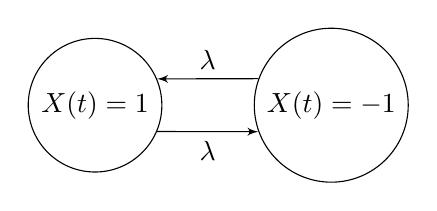
\begin{tikzpicture}
                        % vertices
                            \node[vertex] (1) at (0,0) {$X(t) = 1$};
                            \node[vertex] (2) at (3,0) {$X(t) = -1$};
                        %edges
                        \draw[edge] (1.337) -- (2.200) node[midway, below] {$\lambda$};
                        \draw[edge] (2.160) -- (1.23) node[midway, above] {$\lambda$};
                        \end{tikzpicture}
                    \item $P[X(t_2) = k | X(t_1) = k] = P[\text{even \# of transitions in } (t_1, t_2]] = e^{-\lambda (t_2 - t_1)} \sum_{i = 0}^\infty \frac{(\lambda (t_2 - t_1))^{2j}}{(2j)!}$

                        $= e^{-\lambda (t_2 - t_1)}\frac{e^{\lambda (t_2 - t_1)} + e^{-\lambda (t_2 - t_1)}}{2} = \frac{1 + e^{-2\lambda (t_2 - t_1)}}{2}$
                    \item $\mathit{Cov}(X(t_1), X(t_2)) = \mathbb{E}[X(t_1)X(t_2)] = P[X(t_2) == X(t_1)] - P[X(t_2) \not = X(t_1)] = e^{-2\lambda (t_2 - t_1)}$
                    \item $N(t) = \lim_{n \rightarrow \infty} \frac{1}{\sqrt{n}} \sum_{i=1}^n X_i(t)$
                    \item By Central limit Theorem for stochastic process $\rightarrow N(t)$ is a Gaussian Process
                        \begin{itemize}
                            \item $\mathbb{E}[N(t)] = 0$
                            \item $\mathit{Cov}(N(t_1), N(t_2)) = \lim_{n \rightarrow \infty} \frac{1}{n} \mathit{Cov}(\sum_{i=1}^n X_i(t_1), \sum_{i=1}^n X_i(t_2)) = e^{-2\lambda (t_2 - t_1)}$
                        \end{itemize}
                    \item $N(t)$ is a Stationary Ornstein-Uhlenbeck Process with $\beta = 2 \lambda$ and $\sigma^2 = 2 \beta$
                \end{itemize}
            \item Definition
                \begin{itemize}
                    \item $V_s(t) = \frac{\sigma e^{-\beta t}}{\sqrt{2\beta }} B(e^{2\beta t})$, where $B(t)$ is a Brownian motion
                \end{itemize}
            \item Property
                \begin{itemize}
                    \item Expectation and Covariance
                        \begin{itemize}
                            \item $\mathbb{E}[V_s(t)] = 0$
                            \item $\mathit{Cov}(V_s(t_1), V_s(t_2)) = \frac{\sigma^2}{2\beta} e^{-\beta(t_2 - t_1)}$

                                Proof: $\mathit{Cov}(V_s(t_1), V_s(t_2)) = \frac{\sigma^2}{2\beta} e^{-\beta(t_1 + t_2)} e^{2\beta t_1}$
                                $= \frac{\sigma^2}{2\beta} e^{-\beta(t_2 - t_1)}$
                            \item $\mathit{Var}(V_s(t)) = \frac{\sigma^2}{2\beta}$
                        \end{itemize}
                \end{itemize}
        \end{itemize}
    \item Ornstein-Uhlenbeck Process $V(t)$
        \begin{itemize}
            \item Interpretation
                \begin{enumerate}
                    \item A stationary Ornstein-Uhlenbeck Process with bias
                    \item Ornstein-Uhlenbeck Position Process is approximately a Brownian motion $\rightarrow$ Ornstein-Uhlenbeck Process is approximately the velocity of a Brownian motion

                        Proof
                        \begin{itemize}
                            \item $P(t) = \int_0^t V(x) dx$

                                $= \int_0^t V(0) e^{-\beta x} + \sigma \int_{u=0}^x e^{-\beta (x-u)} d B(u) dx$

                                $= V(0) \frac{1 - e^{-\beta t}}{\beta} + \sigma \int_{u=0}^t \int_u^t e^{-\beta (x-u)} d x d B(u)$

                                $= V(0) \frac{1 - e^{-\beta t}}{\beta} + \frac{\sigma}{\beta} \int_{u=0}^t (1 - e^{-\beta (t-u)}) d B(u)$
                                $= V(0) \frac{1 - e^{-\beta t}}{\beta} + \frac{\sigma}{\beta} B(t) - \frac{\sigma}{\beta} \int_{u=0}^t e^{-\beta (t-u)} d B(u)$
                            \item When $t \rightarrow \infty$, $P(t) \rightarrow \frac{\sigma}{\beta} B(t) - \frac{1}{\beta}V(t) = \frac{\sigma}{\beta} B(t)$
                        \end{itemize}
                \end{enumerate}
            \item Definition
                \begin{enumerate}
                    \item $V(t) = V(0) e^{-\beta t} + \frac{\sigma e^{-\beta t}}{\sqrt{2\beta }} B(e^{2\beta t} - 1)$, where $B(t)$ is a Brownian motion
                    \item $V(t) = V(0) e^{-\beta t} + \sigma \int_{u=0}^t e^{-\beta (t-u)} d B(u)$, where $B(t)$ is a Brownian motion
                    \item $dV(t) = -\beta V(t) dt + \sigma d B(t)$, where $B(t)$ is a Brownian motion
                \end{enumerate}
                Equivalance
                \begin{itemize}
                    \item between Definition 1 and 2
                        \begin{enumerate}
                            \item by definition 2: $\mathbb{E}[V(t)] = V(0) e^{-\beta t}$
                            \item by definition 2: $\mathit{Cov}(V(t_1), V(t_2)) = \frac{\sigma^2}{2\beta} e^{-\beta(t_2 - t_1)} (1 - e^{-2\beta t_1})$

                                Proof
                                \begin{itemize}
                                    \item $\mathit{Cov}(V(t_1), V(t_2))$
                                        $= \sigma^2 \int_{u=0}^{t_1} e^{-\beta(t_1 - u)} e^{-\beta(t_2 - u)} du$
                                        $= \frac{\sigma^2}{2\beta} e^{-\beta(t_2 - t_1)} (1 - e^{-2\beta t_1})$
                                \end{itemize}
                            \item Same Definition:
                                \begin{itemize}
                                    \item Gaussian Process is determined by its expectation and covariance
                                \end{itemize}
                            \item Different random variable 
                                \begin{itemize}
                                    \item definition use different simulation point of $B(t) \rightarrow$ $e^{2 \beta t} - 1$ and $t$
                                \end{itemize}
                        \end{enumerate}
                    \item from Definition 2 to 3
                        \begin{itemize}
                            \item derived by It\^{o} Lemma
                        \end{itemize}
                    \item from Definition 3 to 2
                        \begin{itemize}
                            \item Suppose $E(t) = e^{\beta t}V(t)$
                            \item $dE(t) = \beta E(t) dt + e^{\beta t}d V(t)$
                            $= \sigma e^{\beta t} d B(t)$
                            \item $E(t) = E(0) + \sigma \int_{x=0}^te^{\beta x} dB(x)$
                            \item $V(t) = V(0) e^{-\beta t} + \sigma \int_{x=0}^te^{-\beta (t-x)} dB(x)$
                        \end{itemize}
                \end{itemize}
            \item Property
                \begin{itemize}
                    \item Stationary and Markovian: $V(t_1 + t_2) = V(t_1) e^{-\beta t_2} + \frac{\sigma e^{-\beta t_2}}{\sqrt{2\beta }} B(e^{2\beta t_2} - 1)$

                        Proof
                        \begin{itemize}
                            \item $V(t_1 + t_2)$
                                $= V(0) e^{-\beta (t_1 + t_2)} + \frac{\sigma e^{-\beta (t_1 + t_2)}}{\sqrt{2\beta }} B(e^{2\beta (t_1 + t_2)} - 1)$

                                $= V(t_1) e^{-\beta t_2} + \frac{\sigma e^{-\beta (t_1 + t_2)}}{\sqrt{2\beta }} [B(e^{2\beta (t_1+t_2)} - 1) - B(e^{2\beta t_1} - 1)]$

                                $= V(t_1) e^{-\beta t_2} + \frac{\sigma e^{-\beta t_2}}{\sqrt{2\beta }} B(e^{2\beta (t_2)} - 1)$
                        \end{itemize}
                    \item Increment
                        \begin{itemize}
                            \item $\mathbb{E}[V(t_2) - V(t_1)|V(t_1)] = V(t_1) (e^{-\beta (t_2 - t_1)} - 1)$

                                Proof: $\mathbb{E}[V(t_2) - V(t_1)|V(t_1)]$

                                $= \mathbb{E}[V(t_1) e^{-\beta (t_2 - t_1)} + \frac{\sigma e^{-\beta (t_2 - t_1)}}{\sqrt{2\beta }} B(e^{2\beta ((t_2 - t_1))} - 1) - V(t_1) | V(t_1)]$
                                $= V(t_1) (e^{-\beta (t_2 - t_1)} - 1)$
                            \item $\mathit{Var}(V(t_2) - V(t_1)|V(t_1)) = \frac{\sigma^2}{2\beta} (1 - e^{-2\beta (t_2 - t_1)})$

                                Proof: $\mathit{Var}(V(t_2) - V(t_1)|V(t_1))$

                                $= \mathit{Var}(V(t_1) e^{-\beta (t_2 - t_1)} + \frac{\sigma e^{-\beta (t_2 - t_1)}}{\sqrt{2\beta }} B(e^{2\beta (t_2 - t_1)} - 1) - V(t_1) | V(t_1))$

                                $= \frac{\sigma^2 e^{-2\beta (t_2 - t_1)}}{2\beta} (e^{2\beta (t_2 - t_1)} - 1)$
                                $= \frac{\sigma^2}{2\beta} (1 - e^{-2\beta (t_2 - t_1)})$
                        \end{itemize}
                    \item Expectation and Covariance
                        \begin{itemize}
                            \item $\mathbb{E}[V(t)] = V(0)e^{-\beta t}$
                            \item $\mathit{Cov}(V(t_1), V(t_2)) = \frac{\sigma^2}{2\beta} e^{-\beta(t_2 - t_1)} (1 - e^{-2\beta t_1})$

                                Proof: $\mathit{Cov}(V(t_1), V(t_2)) = \frac{\sigma^2}{2\beta} e^{-\beta(t_1 + t_2)} (e^{2\beta t_1} - 1)$

                                $= \frac{\sigma^2}{2\beta} e^{-\beta(t_2 - t_1)} (1 - e^{-2\beta t_1})$
                            \item $\mathit{Var}(V(t)) = \frac{\sigma^2}{2\beta} (1 - e^{-2\beta t})$
                        \end{itemize}
                \end{itemize}
        \end{itemize}
    \item Ornstein-Uhlenbeck Position Process $P(t)$

        Definition
        \begin{itemize}
            \item $P(t) = \int_0^t V(x) dx$
        \end{itemize}
        Interpretation
        \begin{itemize}
            \item the integral of Ornstein-Uhlenbeck Process
        \end{itemize}
\end{itemize}

\section{Stochastic Differential Equation (SDE)}
\begin{itemize}
    \item Interpretation
        \begin{itemize}
            \item Given a diffusion process $f(x, B(x))$ such that $d f(x, B(x)) = \mu(x, B(x)) dx + \sigma(x, B(x)) d B(x)$ , iff the following three properties are satisfied
                \begin{enumerate}
                    \item Continuity: $\forall \epsilon > 0, P[|f(x+h, B(x+h)) - f(x, B(x))| > \epsilon] = o(h)$
                    \item $\mathbb{E}[f(x+h, B(x+h)) - f(x, B(x))| f(x, B(x))] = \mu(x, B(x)) h + o(h)$

                        By $\mathbb{E}[d f(x, B(x))] = \mathbb{E}[\mu(x, B(x)) dx + \sigma(x, B(x)) d B(x)]$
                    \item $\mathbb{E}[(f(x+h, B(x+h)) - f(x, B(x)))^2| f(x, B(x))] = \sigma^2(x, B(x)) h + o(h)$

                        By $\mathbb{E}[(d f(x, B(x)))^2] = \mathbb{E}[(\mu(x, B(x)) dx + \sigma(x, B(x)) d B(x))^2]$
                \end{enumerate}
        \end{itemize}
    \item Definition
        \begin{itemize}
            \item $d f(x, B(x)) = \mu(x, B(x)) dx + \sigma(x, B(x)) d B(x)$
                \begin{itemize}
                    \item $\mu(x, B(x))$: drift term
                    \item $\sigma(x, B(x))$: variance term
                \end{itemize}
            \item $f(t, B(t)) - f(0, B(0)) = \int_0^t \mu(x, B(x)) dx + \int_{x=0}^t \sigma(x, B(x)) d B(x)$
                \begin{itemize}
                    \item $\int_0^t \mu(x, B(x)) dx$: normal integral
                    \item $\int_0^t \sigma(x, B(x)) d B(x)$: It\^{o} integral
                \end{itemize}
        \end{itemize}
    \item Property:

        Martingale Representation Theorem: Martingale diffusion process has drift term of 0
        \begin{itemize}
            \item Since $\mathbb{E}[f(x+h, B(x+h)) - f(x, B(x))| f(x, B(x))] = 0$
        \end{itemize}
    \item Solve SDE

        Strong Solution: closed form of $f(x, B(x))$
        \begin{itemize}
            \item General Linear SDE: $d f(x, B(x)) = (\mu_1(t) f(x, B(x)) + \mu_2(t))dx + (\sigma_1(t) f(x, B(x)) + \sigma_2(t)) d B(x)$
            \item Steps
                \begin{enumerate}
                    \item solve $f_1(x, B(x))$ such that $d f_1(x, B(x)) = \mu_1(t) f_1(x, B(x)) dx + \sigma_1(t) f_1(x, B(x)) d B(x)$
                        \begin{itemize}
                            \item Suppose $f_2(x, B(x)) = \ln f_1(x, B(x))$
                            \item $d f_2(x, B(x)) = (\mu_1(x) - \frac{1}{2}\sigma_1^2(x)) dx + \sigma_1 d B(x)$
                            \item $f_2(t, B(t)) = \int_0^t (\mu_1(x) - \frac{1}{2}\sigma_1^2(x)) dx + \int_{x=0}^t \sigma_1(x) d B(x)$
                            \item $f_1(t, B(t)) = e^{\int_0^t (\mu_1(x) - \frac{1}{2}\sigma_1^2(x)) dx + \int_{x=0}^t \sigma_1(x) d B(x)}$
                        \end{itemize}
                    \item solve $f_3(x, B(x))$ such that $f_3(x, B(x)) = \frac{f(x, B(x))}{f_1(x, B(x))}$
                        \begin{itemize}
                            \item $d f_3(x, B(x)) = d(\frac{f(x, B(x))}{f_1(x, B(x))}) = \frac{\mu_2(x) - \sigma_1(x) \sigma_2(x)}{f_1(x, B(x))} dx + \frac{\sigma_2(x)}{f_1(x, B(x))} d B(x)$
                            \item $f_3(t, B(t)) = \int_0^t \frac{\mu_2(x) - \sigma_1(x) \sigma_2(x)}{f_1(x, B(x))} dx + \int_{x=0}^t \frac{\sigma_2(x)}{f_1(x, B(x))} d B(x)$
                        \end{itemize}
                    \item $f(x, B(x)) = f_1(x, B(x)) f_3(x, B(x))$
                \end{enumerate}
        \end{itemize}
        Weak Solution: distribution of $f(x, B(x))$ at specific $x$
        \begin{itemize}
            \item Given $f(x, B(x))$ such that $d f(x, B(x)) = \mu(x, B(x)) dx + \sigma(x, B(x)) d B(x)$
            \item Kolmogorov forward diffusion:
                \begin{itemize}
                    \item Suppose $F(x, B(x))$ is the PDF of $f(x, B(x))$
                    \item $F(x, B(x))$ satisfy $\frac{\partial F}{\partial x} = -\frac{\partial \mu(x, B(x)) F}{\partial B(x)} + \frac{1}{2} \frac{\partial^2 \sigma^2(x, B(x)) F}{\partial B^2(x)}$
                \end{itemize}
        \end{itemize}
        Simulation
    \item Example

        Bessel
        \begin{itemize}
            \item $R(t) = ||(B_1(t), B_2(t)|| = \sqrt{B_1^2(t) + B_2^2(t)}$
            \item $d R(t) = \frac{B_1(t)}{R(t)} dB_1(t) + \frac{B_2(t)}{R(t)} dB_2(t) + \frac{1}{2 R(t)} dt$
                \begin{itemize}
                    \item $d R(t) = \frac{B_1(t)}{R(t)} dB_1(t) + \frac{B_2(t)}{R(t)} dB_2(t) + \frac{B_2^2(t)}{2 R^3(t)} (dB_1(t))^2 + \frac{B_1^2(t)}{2 R^3(t)} (dB_2(t))^2 + \frac{-B_1(t)B_2(t)}{R^3(t)} dB_1(t) dB_2(t)$
                    \item $dB_1(t) dB_2(t)$ converge to $0$ in mean square
                \end{itemize}
            \item $\mathbb{E}[d R(t)] = \frac{1}{2 R(t)} dt$
            \item $\mathbb{E}[(d R(t))^2] = dt$
            \item $d R(t) = \frac{1}{2 R(t)} dt + d B(t)$
        \end{itemize}
        Brownian motion with drift
        \begin{itemize}
            \item $d R(t) = \mu dt + \sigma d B(t)$
            \item $R(t) = \mu t + \sigma B(t)$
        \end{itemize}
        Geometric Brownian motion
        \begin{itemize}
            \item $d R(t) = \mu R(t) dt + \sigma R(t) d B(t)$
            \item Suppose $Y(t) = \ln R(t)$
            \item $d Y(t) = \frac{1}{R(t)} d R(t) + \frac{-1}{R^2(t)} (dR(t))^2$
            \item $d Y(t) = \mu dt - \frac{\sigma^2}{2} dt + \sigma dB(t)$
            \item $Y(t) = Y(0) + (\mu - \frac{\sigma^2}{2})t + \sigma B(t)$
            \item $R(t) = R(0)e^{(\mu - \frac{\sigma^2}{2})t + \sigma B(t)}$
        \end{itemize}
\end{itemize}

\end{document}
